% !TEx TS-program = pdflatex
% !TEx encoding = UTF-8 Unicode

% This is a simple template for a LaTex document using the "article" class.
% See "book", "report", "letter" for other types of document.

%\documentclass[14pt]{extarticle} % use larger type; default would be 10pt
%\renewcommand{\baselinestretch}{1.5}
\documentclass[12pt]{article}

%Mikkel bibtex
%\usepackage[maxbibnames=99]{biblatex}
\usepackage{natbib}
\usepackage[nottoc,notlof,notlot]{tocbibind} 
\renewcommand\bibname{References}
\bibpunct{(}{)}{;}{a}{}{;}
\usepackage{breakcites}
%images
\usepackage{graphicx,xcolor}
\graphicspath{ {images/} }
\usepackage[algoruled]{algorithm2e}
\usepackage[pagebackref=false,breaklinks=true]{hyperref} % link colors
\hypersetup{
    colorlinks=true,
    citecolor=black,
    filecolor=black,
    linkcolor=black,
    urlcolor=black,
    %pdfpagemode=UseNone, % comment out bookmarks and use this line
    bookmarksopen=true,
    pdfstartview=FitH
}
\usepackage{caption,threeparttable}

%\usepackage[utf8]{inputenc} % set input encoding (not needed with xeLaTex)

\usepackage{amsthm,amsmath}
\usepackage{bbm}
\usepackage{amsfonts}%
\usepackage{amssymb}%
%%% Examples of Article customizations
% These packages are optional, depending whether you want the features they provide.
% See the LaTex Companion or other references for full information.

%%% PAGE DIMENSIONS
\usepackage{geometry} % to change the page dimensions
%\geometry{a4paper} % or letterpaper (US) or a5paper or....
 \geometry{top = 1in, left = 1in, bottom = 1in, right = 1in} % for example, change the margins to 2 inches all round
% \geometry{landscape} % set up the page for landscape
%   read geometry.pdf for detailed page layout information

\usepackage{graphicx} % support the \includegraphics command and options
\usepackage{framed}
\usepackage{caption}
\usepackage{subcaption}

% \usepackage[parfill]{parskip} % Activate to begin paragraphs with an empty line rather than an indent

%%% PACKAGES
\usepackage{booktabs} % for much better looking tables
\usepackage{array} % for better arrays (eg matrices) in maths
\usepackage{paralist} % very flexible & customisable lists (eg. enumerate/itemize, etc.)
\usepackage{verbatim} % adds environment for commenting out blocks of text & for better verbatim
%\usepackage{subfig} % make it possible to include more than one captioned figure/table in a single float
% These packages are all incorporated in the memoir class to one degree or another...

%%% HEADERS & FOOTERS
%\usepackage{fancyhdr} % This should be set AFTER setting up the page geometry
%\pagestyle{fancy} % options: empty , plain , fancy
%\renewcommand{\headrulewidth}{0pt} % customise the layout...
%\lhead{}\chead{}\rhead{}
%\lfoot{}\cfoot{\thepage}\rfoot{}

%%% SECTION TITLE APPEARANCE
%\usepackage{sectsty}
%\allsectionsfont{\sffamily\mdseries\upshape} % (See the fntguide.pdf for font help)
% (This matches ConText defaults)

%%% ToC (table of contents) APPEARANCE
%\usepackage[nottoc,notlof,notlot]{tocbibind} % Put the bibliography in the ToC
%\usepackage[titles,subfigure]{tocloft} % Alter the style of the Table of Contents
%\renewcommand{\cftsecfont}{\rmfamily\mdseries\upshape}
%\renewcommand{\cftsecpagefont}{\rmfamily\mdseries\upshape} % No bold!
\usepackage{lipsum}
\usepackage{setspace}
\renewcommand{\baselinestretch}{1.5}
\usepackage[singlelinecheck=false]{caption}
\usepackage{tabularx}
\usepackage{tikz}

\usepackage{multicol}
\usepackage{multirow}

\hfuzz=40pt % get rid of that overfull warning
\hbadness=7000 % get rid of that underfull warning

%---------------------------------------------

\newtheorem{theorem}{Theorem}
\newtheorem{assump}{Assumption}
\newtheorem{assump*}{Assumption}[section]
\newcommand{\assumpautorefname}{Assumption} % for autoref
\newtheorem{lemma}{Lemma}
\newcommand{\lemmaautorefname}{Lemma}
\newtheorem{corollary}{Corollary}
\newcommand{\corollaryautorefname}{Corollary}
\newtheorem{proposition}{Proposition}
\newcommand{\propositionautorefname}{Proposition}
\newcommand{\thistheoremname}{}

% custom assumption name
\newcommand{\namedassumpinnerautorefname}{Assumption}
\newtheorem{namedassumpinner}{Assumption}
\newenvironment{namedassump}[1]{%
  \renewcommand\thenamedassumpinner{#1}%
  \namedassumpinner
}{\endnamedassumpinner}

\theoremstyle{definition}
\newtheorem{definition}{Definition}
\newcommand{\definitionautorefname}{Definition}
\newtheorem{example}{Example}
\newcommand{\exampleautorefname}{Example}
\newtheorem{remark}{Remark}
\newcommand{\remarkautorefname}{Remark}

\renewcommand{\algorithmautorefname}{Algorithm}
\def\equationautorefname~#1\null{(#1)\null} % for autoref to work as eqref

\newtheorem{myexp}{Example}

\newenvironment{myexpcont}
{\addtocounter{myexp}{-1}\begin{myexp}{\textit{\textbf{{(continued)}}}}}
  {\end{myexp}}


%---------------------------------------------

\def\indep{\perp\!\!\!\perp}
\newcommand{\argmax}{\operatornamewithlimits{argmax}}
\newcommand{\argmin}{\operatornamewithlimits{argmin}}
\newcommand{\plim}{\text{plim}\,}
\newcommand{\cov}{\text{Cov}}
\newcommand{\var}{\text{Var}}
\newcommand{\E}{{\bf E}}
\newcommand{\R}{\mathbb{R}}
\newcommand{\N}{\mathbb{N}}
\newcommand{\prob}{\mathbf{P}}
\newcommand{\ind}{\bm{1}}
\newcommand{\plimarrow}{\stackrel{p}\longrightarrow}
\newcommand{\dlimarrow}{\stackrel{d}\longrightarrow}
\newcommand{\F}{\mathcal{F}}
\newcommand{\zero}{\bm{0}}
\newcommand{\equivslash}{\mathclose{}/\mathopen{}}
\newcommand*{\medcap}{\mathbin{\scalebox{1.5}{\ensuremath{\cap}}}}
\newcommand*{\medcup}{\mathbin{\scalebox{1.5}{\ensuremath{\cup}}}}
\def\citeapos#1{\citeauthor{#1}'s (\citeyear{#1})}
\providecommand{\abs}[1]{\lvert#1\rvert} 
\providecommand{\norm}[1]{\lVert#1\rVert}
\DeclareMathOperator*{\esup}{ess\,sup}
\DeclareMathOperator*{\einf}{ess\,inf}
\let\oldemptyset\emptyset
\let\emptyset\varnothing

%---------------------------------------------

%\usepackage[colorlinks]{hyperref}
%\hypersetup{allcolors=blue}
%%% END Article customizations
%%% The "real" document content comes below...

\title{Identifying Socially Disruptive Policies} 
\author{Eric Auerbach\footnote{Department of Economics, Northwestern University. E-mail: eric.auerbach@northwestern.edu.} \and Yong Cai \footnote{Department of Economics, Northwestern University. E-mail: yongcai2023@u.northwestern.edu.\newline We thank Hossein Alidaee, Jon Auerbach, Lori Beaman, Vivek Bhattacharya, Stephane Bonhomme, Federico Bugni, Ivan Canay, Matias Cattaneo, Ben Golub, Bryan Graham, Joel Horowitz, Gaston Illanes, Guido Imbens, Chuck Manski, Roger Moon, Rob Porter, Chris Udry, Takuya Ura, and Martin Weidner  for helpful feedback. A version of this paper was previously titled, ``Heterogeneous Treatment Effects for Networks, Panels, and other Outcome Matrices.''  }}
 \date{\parbox{\linewidth}{\centering%
  \today\endgraf}} 
%\date{}

\begin{document}
\maketitle

\begin{abstract} \setstretch{1}\noindent
Social disruption occurs when a policy creates or destroys many network connections between agents. It is a costly side effect of many interventions and so a growing empirical literature recommends measuring and accounting for social disruption when evaluating the welfare impact of a policy. However, there is currently little work characterizing what can actually be learned about social disruption from data in practice. In this paper, we consider the problem of identifying social disruption in a research design that is popular in the literature. We provide two sets of identification results. First, we show that social disruption is not generally point identified, but informative bounds can be constructed using the eigenvalues of the network adjacency matrices observed by the researcher. Second, we show that point identification follows from a theoretically motivated monotonicity condition, and we derive a closed form representation. We apply our methods in two empirical illustrations and find large policy effects that otherwise might be missed by alternatives in the literature.   \looseness=-1 
\end{abstract}


%----------------------------------------------------------------------
\section{Introduction}
%----------------------------------------------------------------------

Many policies are socially disruptive in that they alter a substantial fraction of agents' social or economic connections. Since networks determine a wide range of economic activities, disrupting them can be harmful. For example, \cite{carrell2013natural} study a change in classroom composition that was supposed to improve academic performance but instead segregated students which exacerbated inequality. \cite{barnhardt2017moving} analyze an antipoverty program that was intended to provide economic opportunity but instead isolated participants which led to financial insecurity. Both policies were well intentioned but, because they were socially disruptive, ultimately hurt the agents that they were designed to help.\looseness=-1 

In light of these and other examples, a growing literature recommends measuring and accounting for social disruption when evaluating the welfare impact of a policy \citep[see, for instance,][]{banerjee2021changes,jackson2021inequality}. But identifying social disruption from data is not always straightforward in practice. Economists typically characterize the disruptive impact of a policy by comparing the average number of connections between agents with and without it. While easy to compute, comparing averages generally understates social disruption. The reason for this is that economic policies usually have heterogeneous effects: they create some connections and destroy others. If the amount of created connections is roughly the same as the amount of destroyed connections, then the average difference will be small, even when the total number of connections affected by the policy is not.\footnote{This disruption is policy relevant. It represents actual relationships that are upended, requiring time and resources to replace. The literature shows that new connections may be of lower quality, associated with less trust, communication, peer influence, etc. As a result, this disruption negatively impacts welfare, even when the average number of connections with and without the policy is similar.} \looseness=-1 


In this paper, we go beyond comparing averages and consider the problem of separately identifying the amount of connections created and the amount of connections destroyed by a policy. We focus on a research design that is popular in the literature. Agents are first randomly (or as good as randomly) assigned to one of two groups. The policy is implemented in one of the groups but not the other. The agents in each group then interact and report their connections. Versions of this design are considered, for example, by \cite{carrell2013natural,feigenberg2013economic,cai2015social,bajari2021multiple,banerjee2021changes,comola2021treatment,hess2021development,johari2022experimental}. \looseness=-1 

Our first contribution is to propose a new framework to characterize the impact of a policy on the structure of a network in a randomized experiment. We do not specify an econometric model of link formation. Instead, we use the classical implication of random assignment, that the agents in the group subjected to the policy form connections that are in some sense representative of what the agents in the group not subjected to the policy would have realized had they been subjected to the policy. Formalizing this condition in the context of network data is not standard in econometrics, however, and our framework builds on ideas from the graph theory and operations research literatures \cite[see, generally,][]{lovasz2012large,cela2013quadratic}.  \looseness=-1 

Our second contribution is to derive two new sets of identification results. In the first set of results, we show that under no additional assumptions the amount of connections created or destroyed by a policy is partially identified. Sharp bounds on the identified set are given by a quadratic assignment problem (QAP), but these bounds are analytically and computationally intractable. Instead, we propose conservative outer bounds based on intersecting several relaxations of the QAP. These bounds are formed by simple rearrangements of the eigenvalues of the networks observed from the experiment, and so are straightforward to analyze and compute. In the second set of results, we give a sufficient condition for point identification. Our condition is a monotonicity assumption that is strong, but motivated from the network theory literature. Under this condition, the amount of social disruption is given by a difference in network eigenvalues that is also straightforward to analyze and compute. Though not the focus of our paper, sufficient conditions for consistent estimation and valid inference can be found in the online appendix. An R package for implementation can be found at \url{https://github.com/yong-cai/MatrixHTE}.  \looseness=-1 

We demonstrate our methodology with two empirical illustrations. The first illustration uses data from \cite{banerjee2021changes}. Villages participate in a microfinance program and the network connections are informal risk sharing links between households. The authors compare the average number of connections between villages that do and do not participate and find that participation is associated with a one percent decrease in connections. We find disruptive effects that are nine to twenty one times larger using our bounds. The second illustration uses data from \cite{athey2011comparing}. Plots of timberland are randomly assigned to a sealed or open auction format and the network connections are bids on the plots made by loggers and mills. The authors compare the average number of bids across the two formats and find that the sealed bid format encourages a small fraction of firms to participate. We find disruptive effects that are six to twenty three times larger using our bounds.  \looseness=-1 

Our paper relates to two relatively new literatures on endogenous network formation and partial identification with network data \cite[see, generally, reviews by][]{bramoulle2020peer,graham2020network,molinari2020microeconometrics}. Most of this work focuses on recovering the structural parameters of a social interaction or network formation model, rather than identifying specific network statistics. Two exceptions we know of are \cite{chandrasekhar2011econometrics,thirkettle2019identification}. While these authors focus on identifying centrality measures from sampled networks, our interest is in social disruption from an experiment.  \looseness=-1 

Our paper also relates to an older literature on Frechet-Hoeffding-Makarov bounds \citep{hoeffding1940masstabinvariante,frechet1951tableaux,makarov1982estimates} and quantile treatment effects \citep{doksum1974empirical,lehmann1975nonparametrics,whitt1976bivariate}. See, for instance, \cite{manski1997mixing,manski2003partial,heckman1997making,bitler2006mean,firpo2007efficient,fan2010sharp,tamer2010partial,abadie2018econometric,masten2018identification,masten2020inference,firpo2019partial,frandsen2021partial} for work in econometric program evaluation. However, the structure of our identification problem is fundamentally different, introducing challenges not present in this literature. Intuitively, what distinguishes our framework is that while agents are individually assigned to policies, connections are measured between pairs of agents.\footnote{This is sometimes called ``double randomization,'' see \cite{graham2011econometric,graham2014complementarity,bajari2021multiple,johari2022experimental} for related research designs, but fundamentally different identification problems.} It turns out that this distinction substantially alters the identification problem. Standard results are not generally valid and standard tools when naively applied often fail to identify any social disruption. We provide intuition as to how our problem is different and why our methodology is more appropriate in Section 2. Our formal framework and results are in Sections 3 and 4, with some extensions in Section 5. Two empirical illustrations are in Section 6. Proofs are in the appendix. Additional details are in the online appendix at \url{https://yong-cai.github.io/MatrixHTE/onlineAppendix.pdf}.  \looseness=-1  


%----------------------------------------------------------------------
\section{An illustration of the main identification problem}
%----------------------------------------------------------------------
This section provides a simplified illustration of the main identification problem, deferring the general framework and results to Sections 3 and 4. We focus on identifying the magnitude of connections destroyed by a change in policy. The problem similar in spirit to that of bounding the joint distribution of two random variables using their marginals originally considered by \cite{hoeffding1940masstabinvariante,frechet1951tableaux}. However, our problem has a fundamentally different structure. We give an example where naively applying the bounds from this literature fails to identify any social disruption. Our methodology does. \looseness=-1  

\subsection{A simplified setup}
To learn about the disruptive impact of a new policy, we conduct an experiment where we randomly assign $N$ agents to a treatment group and $N$ agents to a control group. We implement the new policy in group $1$ and maintain the status quo in group $0$. For example, the new policy could be that every agent in the group participates in an antipoverty program. The status quo could be that no agent participates. The $N$ agents in the treatment group interact and form one network. The $N$ agents in the control group interact and form another network. Taking the size of the two groups to be the same simplifies our illustration, but is not necessary for the general framework. \looseness=-1  

We use potential outcome notation. Let policy $1$ refer to the new policy, policy $0$ refer to the status quo, group $1$ refer to the treatment group, and group $0$ refer to the control group. Then $Y_{ij,s}(t)$ is the potential connection between agents $i$ and $j$ in group $s$ under policy $t$. That is, $Y_{ij,s}(t)$ describes what the connection between agents $i$ and $j$ in group $s$ would be if policy $t$ were implemented in that group. $Y_{ij,s}(t)$ is observed if and only if $s = t$. To simplify our illustration, we assume that the networks are unweighted and undirected so that $Y_{ij,s}(t) \in \{0,1\}$. Weighted and directed networks are allowed in the general framework.   \looseness=-1  

For this illustration, the parameter of interest is the number of network connections between the $N$ agents assigned to the control group that would be destroyed by implementing the new policy in that group. That is, 
\begin{align}\label{param}
\frac{1}{2}\sum_{i,j = 1}^{N}(1-Y_{ij,0}(1))Y_{ij,0}(0). 
\end{align}
The problem is that $Y_{ij,0}(1)$ is not observed. Without additional assumptions, $Y_{ij,0}(1)$ could take any value in $\{0,1\}$ so that the identified set for (\ref{param}) is 
\begin{align}\label{paramset}
\left\{\theta \in \mathbb{N} : \theta = \frac{1}{2}\sum_{i,j = 1}^{N}M_{ij}Y_{ij,0}(0) \text{ for any } M_{ij} = M_{ji} \in \{0,1\}\right\}.
\end{align}
Since (\ref{paramset}) is often too large to be informative, the idea is to leverage the assumption that the agents are randomized to the treatment and control groups to refine it.  \looseness=-1  

\begin{myexp}
A toy example with $N = 6$ is illustrated in Figure 1. The six agents assigned to the treatment group form a line. The six agents assigned to the control group form a star.  There are five connections between the agents in the control group out of a possible total of fifteen. Without additional assumptions,  (\ref{paramset}) says that the number of connections that would be destroyed by implementing the policy in this group is between $0$ and $5$. \looseness=-1  
\end{myexp}

\begin{figure}
\centering


\tikzset{every picture/.style={line width=0.75pt}} %set default line width to 0.75pt        

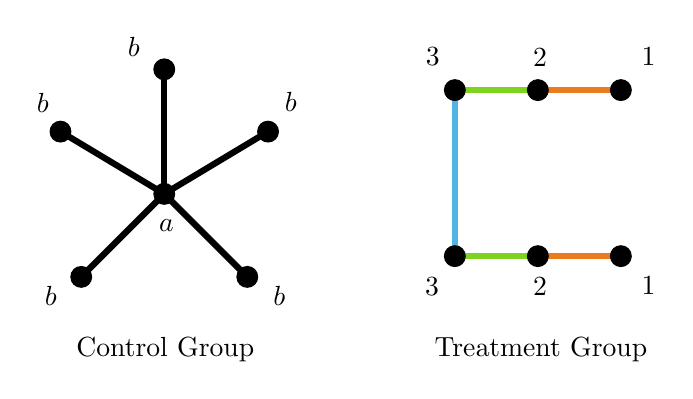
\begin{tikzpicture}[x=0.75pt,y=0.75pt,yscale=-1,xscale=1]
	%uncomment if require: \path (0,242); %set diagram left start at 0, and has height of 242
	
	%Straight Lines [id:da8360249781061426] 
	\draw [color={rgb, 255:red, 235; green, 124; blue, 29 }  ,draw opacity=1 ][line width=2.25]    (285,155) -- (325,155) ;
	%Straight Lines [id:da8158257704190623] 
	\draw [color={rgb, 255:red, 235; green, 124; blue, 29 }  ,draw opacity=1 ][line width=2.25]    (285,75) -- (325,75) ;
	%Straight Lines [id:da7285129998191696] 
	\draw [line width=2.25]    (105,65) -- (105,125) ;
	%Straight Lines [id:da1945257120538626] 
	\draw [line width=2.25]    (65,165) -- (105,125) ;
	%Straight Lines [id:da15064502001286517] 
	\draw [line width=2.25]    (105,125) -- (145,165) ;
	%Straight Lines [id:da8625361583469673] 
	\draw [color={rgb, 255:red, 126; green, 211; blue, 33 }  ,draw opacity=1 ][line width=2.25]    (245,75) -- (285,75) ;
	%Straight Lines [id:da8513199064736671] 
	\draw [color={rgb, 255:red, 126; green, 211; blue, 33 }  ,draw opacity=1 ][line width=2.25]    (245,155) -- (285,155) ;
	%Straight Lines [id:da5064308868951334] 
	\draw [color={rgb, 255:red, 80; green, 181; blue, 227 }  ,draw opacity=1 ][line width=2.25]    (245,75) -- (245,155) ;
	%Shape: Circle [id:dp7020190518871161] 
	\draw  [fill={rgb, 255:red, 0; green, 0; blue, 0 }  ,fill opacity=1 ] (100,65) .. controls (100,62.24) and (102.24,60) .. (105,60) .. controls (107.76,60) and (110,62.24) .. (110,65) .. controls (110,67.76) and (107.76,70) .. (105,70) .. controls (102.24,70) and (100,67.76) .. (100,65) -- cycle ;
	%Shape: Circle [id:dp4472245437398714] 
	\draw  [fill={rgb, 255:red, 0; green, 0; blue, 0 }  ,fill opacity=1 ] (100,125) .. controls (100,122.24) and (102.24,120) .. (105,120) .. controls (107.76,120) and (110,122.24) .. (110,125) .. controls (110,127.76) and (107.76,130) .. (105,130) .. controls (102.24,130) and (100,127.76) .. (100,125) -- cycle ;
	%Shape: Circle [id:dp332527728107481] 
	\draw  [fill={rgb, 255:red, 0; green, 0; blue, 0 }  ,fill opacity=1 ] (60,165) .. controls (60,162.24) and (62.24,160) .. (65,160) .. controls (67.76,160) and (70,162.24) .. (70,165) .. controls (70,167.76) and (67.76,170) .. (65,170) .. controls (62.24,170) and (60,167.76) .. (60,165) -- cycle ;
	%Shape: Circle [id:dp5070907001685069] 
	\draw  [fill={rgb, 255:red, 0; green, 0; blue, 0 }  ,fill opacity=1 ] (140,165) .. controls (140,162.24) and (142.24,160) .. (145,160) .. controls (147.76,160) and (150,162.24) .. (150,165) .. controls (150,167.76) and (147.76,170) .. (145,170) .. controls (142.24,170) and (140,167.76) .. (140,165) -- cycle ;
	%Shape: Circle [id:dp7312361016882203] 
	\draw  [fill={rgb, 255:red, 0; green, 0; blue, 0 }  ,fill opacity=1 ] (240,75) .. controls (240,72.24) and (242.24,70) .. (245,70) .. controls (247.76,70) and (250,72.24) .. (250,75) .. controls (250,77.76) and (247.76,80) .. (245,80) .. controls (242.24,80) and (240,77.76) .. (240,75) -- cycle ;
	%Shape: Circle [id:dp6877519316777763] 
	\draw  [fill={rgb, 255:red, 0; green, 0; blue, 0 }  ,fill opacity=1 ] (320,75) .. controls (320,72.24) and (322.24,70) .. (325,70) .. controls (327.76,70) and (330,72.24) .. (330,75) .. controls (330,77.76) and (327.76,80) .. (325,80) .. controls (322.24,80) and (320,77.76) .. (320,75) -- cycle ;
	%Shape: Circle [id:dp21492882036619276] 
	\draw  [fill={rgb, 255:red, 0; green, 0; blue, 0 }  ,fill opacity=1 ] (320,155) .. controls (320,152.24) and (322.24,150) .. (325,150) .. controls (327.76,150) and (330,152.24) .. (330,155) .. controls (330,157.76) and (327.76,160) .. (325,160) .. controls (322.24,160) and (320,157.76) .. (320,155) -- cycle ;
	%Shape: Circle [id:dp1595771278608995] 
	\draw  [fill={rgb, 255:red, 0; green, 0; blue, 0 }  ,fill opacity=1 ] (240,155) .. controls (240,152.24) and (242.24,150) .. (245,150) .. controls (247.76,150) and (250,152.24) .. (250,155) .. controls (250,157.76) and (247.76,160) .. (245,160) .. controls (242.24,160) and (240,157.76) .. (240,155) -- cycle ;
	%Straight Lines [id:da9822349173412578] 
	\draw [line width=2.25]    (105,125) -- (155,95) ;
	%Shape: Circle [id:dp7709379434514961] 
	\draw  [fill={rgb, 255:red, 0; green, 0; blue, 0 }  ,fill opacity=1 ] (150,95) .. controls (150,92.24) and (152.24,90) .. (155,90) .. controls (157.76,90) and (160,92.24) .. (160,95) .. controls (160,97.76) and (157.76,100) .. (155,100) .. controls (152.24,100) and (150,97.76) .. (150,95) -- cycle ;
	%Shape: Circle [id:dp9939137807167766] 
	\draw  [fill={rgb, 255:red, 0; green, 0; blue, 0 }  ,fill opacity=1 ] (50,95) .. controls (50,92.24) and (52.24,90) .. (55,90) .. controls (57.76,90) and (60,92.24) .. (60,95) .. controls (60,97.76) and (57.76,100) .. (55,100) .. controls (52.24,100) and (50,97.76) .. (50,95) -- cycle ;
	%Straight Lines [id:da9699796513691362] 
	\draw [line width=2.25]    (55,95) -- (105,125) ;
	%Shape: Circle [id:dp9943805701380365] 
	\draw  [fill={rgb, 255:red, 0; green, 0; blue, 0 }  ,fill opacity=1 ] (280,75) .. controls (280,72.24) and (282.24,70) .. (285,70) .. controls (287.76,70) and (290,72.24) .. (290,75) .. controls (290,77.76) and (287.76,80) .. (285,80) .. controls (282.24,80) and (280,77.76) .. (280,75) -- cycle ;
	%Shape: Circle [id:dp0350269156660592] 
	\draw  [fill={rgb, 255:red, 0; green, 0; blue, 0 }  ,fill opacity=1 ] (280,155) .. controls (280,152.24) and (282.24,150) .. (285,150) .. controls (287.76,150) and (290,152.24) .. (290,155) .. controls (290,157.76) and (287.76,160) .. (285,160) .. controls (282.24,160) and (280,157.76) .. (280,155) -- cycle ;
	
	% Text Node
	\draw (106,140.5) node   [align=left] {$\displaystyle a$};
	% Text Node
	\draw (90.38,54) node   [align=left] {$\displaystyle b$};
	% Text Node
	\draw (50.38,174) node   [align=left] {$\displaystyle b$};
	% Text Node
	\draw (160.38,174) node   [align=left] {$\displaystyle b$};
	% Text Node
	\draw (234.38,59) node   [align=left] {$\displaystyle 3$};
	% Text Node
	\draw (234,169.5) node   [align=left] {$\displaystyle 3$};
	% Text Node
	\draw (338.38,169) node   [align=left] {$\displaystyle 1$};
	% Text Node
	\draw (338.38,59) node   [align=left] {$\displaystyle 1$};
	% Text Node
	\draw (286.5,200) node   [align=left] {Treatment Group};
	% Text Node
	\draw (105.5,200) node   [align=left] {Control Group};
	% Text Node
	\draw (286,59.5) node   [align=left] {$\displaystyle 2$};
	% Text Node
	\draw (286,169.5) node   [align=left] {$\displaystyle 2$};
	% Text Node
	\draw (166,80.5) node   [align=left] {$\displaystyle b$};
	% Text Node
	\draw (46.5,81) node   [align=left] {$\displaystyle b$};
	
	
\end{tikzpicture}
\vspace{-6mm}
\caption{A toy example of an experiment. The six agents assigned to the treatment group form a line. The six agents assigned to the control group form a star.}
\label{fig:toyexample_problem}
\end{figure}

\subsection{The main identification assumption}
Our first main contribution is to propose a condition that formalizes how randomization restricts the identified set. Our main identification assumption is that $Y_{0}(1)$ and $Y_{1}(1)$ are \emph{weakly isomorphic}. We defer a formal definition of this condition to Section 3. In words, it says that the frequency of any network configuration such as a link between two agents, a triangle between three agents, a star between six agents, etc. would be the same for the two treatment groups if they were both assigned the new policy. It is a network analog of the conventional assumption that the entries of $Y_{0}(1)$ and $Y_{1}(1)$ have the same empirical distribution. Equality of distribution is a strong but ubiquitous implication of random assignment, see Chapter 7.3 of \cite{manski2009identification} for an in depth discussion. \looseness=-1

As with equality of distribution in a conventional experiment, randomization only generally implies that $Y_{0}(1)$ and $Y_{1}(1)$ are weakly isomorphic in large samples or in expectation. However, to illustrate the main identification problem, we will in this section make the strong and potentially unrealistic assumption that it holds exactly in the realized experiment. What this means is that the configuration of links connecting the $N$ agents in the treatment group describe exactly how the $N$ agents in the control group would be linked under the new policy. Formally, there exists an $N\times N$ permutation matrix $\Pi$, unknown to the researcher, such that  \looseness=-1 
\begin{align}\label{simAss}
Y_{ij,0}(1) = \sum_{k,l=1}^{N}Y_{kl,1}(1)\Pi_{ik}\Pi_{jl}.
\end{align}


Condition (\ref{simAss}) suggests an experiment conducted on $N$ pairs or ``clones'' of agents. One member of each pair is randomly assigned to each group and the counterfactual connection between agents in the control group is given by their clones in the treatment group. If the researcher knows which pairs of agents are clones, then they can  compute (\ref{param}) by simply substituting $Y_{ij,0}(1)$ with $Y_{c_{i}c_{j},1}(1)$ where $c_{i}$ is the identity of $i$'s clone. But the researcher has forgotten this information so that, in principle, any matching between the agents of the treatment and control groups (as represented by some permutation matrix) could be the correct one.  \looseness=-1  

Randomization does not generally imply that (\ref{simAss}) holds exactly in finite samples. Instead, it is an approximation to what randomization does in large samples. The idea that randomization can be characterized by an approximate matching is not original to our paper: an analogous condition plays a key role in the identification arguments of the Frechet-Hoeffding-Makarov bounds and quantile treatment effects literature. See \cite{whitt1976bivariate,heckman1997making} for detailed discussions. What is new in our setting is that the quadratic structure of (\ref{simAss}) makes the problem of identifying social disruption with network data fundamentally different. We discuss this complication in Section 2.2.2 below.   \looseness=-1  

\subsubsection{The identified set under the main identification assumption}
Though condition (\ref{simAss}) is intended to be a large sample approximation, to illustrate its identifying content in this section we suppose it holds exactly. Plugging (\ref{simAss}) into (\ref{param}) implies that the number of links destroyed by the policy is \looseness=-1  
\begin{align*}
\frac{1}{2}\sum_{i,j = 1}^{N}(1-Y_{ij,0}(1))Y_{ij,0}(0) = \frac{1}{2}\sum_{i,j,k,l = 1}^{N}(1-Y_{ij,1}(1))Y_{kl,0}(0)\Pi_{ik}\Pi_{jl}.
\end{align*}
The substitution solves the initial problem that $Y_{0}(1)$ is not known because both $Y_{1}(1)$ and $Y_{0}(0)$ on the right-hand side are observed. However, the right-hand side now depends on the unknown $\Pi$. Since, under (\ref{simAss}), any permutation matrix suggests a number of destroyed links that is consistent with the observed network connections, the identified set is \looseness=-1  
 \begin{align}\label{paramset2}
 \left\{\theta \in \mathbb{N}: \theta = \frac{1}{2}\sum_{i,j,k,l = 1}^{N}(1-Y_{ij,1}(1))Y_{kl,0}(0)P_{ik}P_{jl} \text{ for any permutation matrix } P \right\}.
 \end{align}



\begin{myexpcont}
In the toy example, condition (\ref{simAss}) implies that if the new policy were implemented in the control group, the agents would change their social connections to form a line. Under this assumption, the identified set for the number of connections destroyed by the policy is $\{3,4\}$. The logic behind this result is illustrated in Figure 2. There are three ways up to symmetry to match the six agents in the control group to the six agents in the treatment group. Matching  $a$ in the control group to position $1$ in the treatment group destroys four connections. This is because all five connections in the control group are adjacent to $a$ and $1$ has only one connection in the treatment group. Similarly, matching $a$ to positions $2$ or $3$ destroys three connections. Since these are the only unique matches up to symmetry, the policy must destroy 3 or 4 out of 5 connections ($60$ or $80$ percent). Under  (\ref{simAss}), this example necessarily has a large amount of social disruption. \looseness=-1  
\end{myexpcont}

\begin{figure}
\centering


\tikzset{every picture/.style={line width=0.75pt}} %set default line width to 0.75pt        

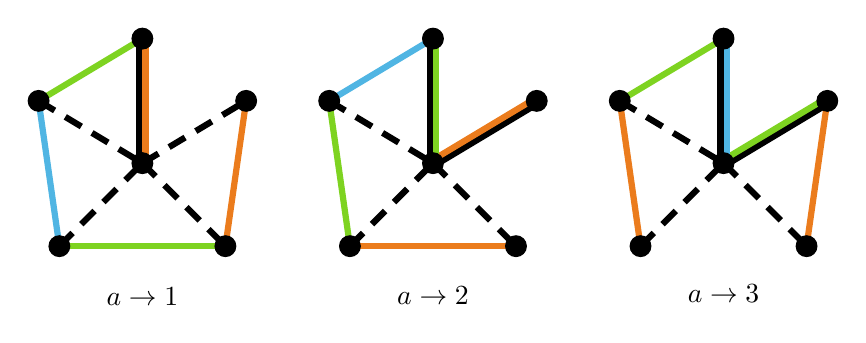
\begin{tikzpicture}[x=0.75pt,y=0.75pt,yscale=-1,xscale=1]
	%uncomment if require: \path (0,242); %set diagram left start at 0, and has height of 242
	
	%Straight Lines [id:da6006307035883517] 
	\draw [color={rgb, 255:red, 235; green, 124; blue, 29 }  ,draw opacity=1 ][line width=2.25]    (315,165) -- (305,95) ;
	%Straight Lines [id:da2628452665477662] 
	\draw [line width=2.25]    (216,126) -- (266,96) ;
	%Straight Lines [id:da7867605309196273] 
	\draw [color={rgb, 255:red, 235; green, 124; blue, 29 }  ,draw opacity=1 ][line width=2.25]    (214,124) -- (264,94) ;
	%Straight Lines [id:da20974090082161245] 
	\draw [color={rgb, 255:red, 235; green, 124; blue, 29 }  ,draw opacity=1 ][line width=2.25]    (125,95) -- (115,165) ;
	%Straight Lines [id:da3642708459455063] 
	\draw [color={rgb, 255:red, 126; green, 211; blue, 33 }  ,draw opacity=1 ][line width=2.25]    (35,165) -- (115,165) ;
	%Straight Lines [id:da2510429813427911] 
	\draw [color={rgb, 255:red, 80; green, 181; blue, 227 }  ,draw opacity=1 ][line width=2.25]    (35,165) -- (25,95) ;
	%Straight Lines [id:da26518610675394505] 
	\draw [color={rgb, 255:red, 126; green, 211; blue, 33 }  ,draw opacity=1 ][line width=2.25]    (25,95) -- (75,65) ;
	%Straight Lines [id:da15555504660860886] 
	\draw [line width=2.25]    (73.5,65) -- (73.5,125) ;
	%Straight Lines [id:da9319742594731747] 
	\draw [color={rgb, 255:red, 235; green, 124; blue, 29 }  ,draw opacity=1 ][line width=2.25]    (76.5,65) -- (76.5,125) ;
	%Straight Lines [id:da5351968154129055] 
	\draw [line width=2.25]  [dash pattern={on 6.75pt off 4.5pt}]  (35,165) -- (75,125) ;
	%Straight Lines [id:da2677247736086712] 
	\draw [line width=2.25]  [dash pattern={on 6.75pt off 4.5pt}]  (75,125) -- (115,165) ;
	%Shape: Circle [id:dp2822714540066722] 
	\draw  [fill={rgb, 255:red, 0; green, 0; blue, 0 }  ,fill opacity=1 ] (70,65) .. controls (70,62.24) and (72.24,60) .. (75,60) .. controls (77.76,60) and (80,62.24) .. (80,65) .. controls (80,67.76) and (77.76,70) .. (75,70) .. controls (72.24,70) and (70,67.76) .. (70,65) -- cycle ;
	%Shape: Circle [id:dp8647332015586298] 
	\draw  [fill={rgb, 255:red, 0; green, 0; blue, 0 }  ,fill opacity=1 ] (70,125) .. controls (70,122.24) and (72.24,120) .. (75,120) .. controls (77.76,120) and (80,122.24) .. (80,125) .. controls (80,127.76) and (77.76,130) .. (75,130) .. controls (72.24,130) and (70,127.76) .. (70,125) -- cycle ;
	%Shape: Circle [id:dp9341805611726252] 
	\draw  [fill={rgb, 255:red, 0; green, 0; blue, 0 }  ,fill opacity=1 ] (30,165) .. controls (30,162.24) and (32.24,160) .. (35,160) .. controls (37.76,160) and (40,162.24) .. (40,165) .. controls (40,167.76) and (37.76,170) .. (35,170) .. controls (32.24,170) and (30,167.76) .. (30,165) -- cycle ;
	%Shape: Circle [id:dp6347309455271312] 
	\draw  [fill={rgb, 255:red, 0; green, 0; blue, 0 }  ,fill opacity=1 ] (110,165) .. controls (110,162.24) and (112.24,160) .. (115,160) .. controls (117.76,160) and (120,162.24) .. (120,165) .. controls (120,167.76) and (117.76,170) .. (115,170) .. controls (112.24,170) and (110,167.76) .. (110,165) -- cycle ;
	%Straight Lines [id:da2354506575862637] 
	\draw [line width=2.25]  [dash pattern={on 6.75pt off 4.5pt}]  (75,125) -- (125,95) ;
	%Shape: Circle [id:dp27440282635206015] 
	\draw  [fill={rgb, 255:red, 0; green, 0; blue, 0 }  ,fill opacity=1 ] (120,95) .. controls (120,92.24) and (122.24,90) .. (125,90) .. controls (127.76,90) and (130,92.24) .. (130,95) .. controls (130,97.76) and (127.76,100) .. (125,100) .. controls (122.24,100) and (120,97.76) .. (120,95) -- cycle ;
	%Shape: Circle [id:dp2742824203776172] 
	\draw  [fill={rgb, 255:red, 0; green, 0; blue, 0 }  ,fill opacity=1 ] (20,95) .. controls (20,92.24) and (22.24,90) .. (25,90) .. controls (27.76,90) and (30,92.24) .. (30,95) .. controls (30,97.76) and (27.76,100) .. (25,100) .. controls (22.24,100) and (20,97.76) .. (20,95) -- cycle ;
	%Straight Lines [id:da5792134404795799] 
	\draw [line width=2.25]  [dash pattern={on 6.75pt off 4.5pt}]  (25,95) -- (75,125) ;
	%Straight Lines [id:da9688758191181335] 
	\draw [color={rgb, 255:red, 235; green, 124; blue, 29 }  ,draw opacity=1 ][line width=2.25]    (175,165) -- (255,165) ;
	%Straight Lines [id:da32600537898081305] 
	\draw [color={rgb, 255:red, 126; green, 211; blue, 33 }  ,draw opacity=1 ][line width=2.25]    (175,165) -- (165,95) ;
	%Straight Lines [id:da8779003930009404] 
	\draw [color={rgb, 255:red, 80; green, 181; blue, 227 }  ,draw opacity=1 ][line width=2.25]    (165,95) -- (215,65) ;
	%Straight Lines [id:da9721333086578243] 
	\draw [line width=2.25]    (213.5,65) -- (213.5,125) ;
	%Straight Lines [id:da2605254490006198] 
	\draw [color={rgb, 255:red, 126; green, 211; blue, 33 }  ,draw opacity=1 ][line width=2.25]    (216.5,65) -- (216.5,125) ;
	%Straight Lines [id:da3689463172698282] 
	\draw [line width=2.25]  [dash pattern={on 6.75pt off 4.5pt}]  (175,165) -- (215,125) ;
	%Straight Lines [id:da3422067536965029] 
	\draw [line width=2.25]  [dash pattern={on 6.75pt off 4.5pt}]  (215,125) -- (255,165) ;
	%Shape: Circle [id:dp41630836475307786] 
	\draw  [fill={rgb, 255:red, 0; green, 0; blue, 0 }  ,fill opacity=1 ] (210,65) .. controls (210,62.24) and (212.24,60) .. (215,60) .. controls (217.76,60) and (220,62.24) .. (220,65) .. controls (220,67.76) and (217.76,70) .. (215,70) .. controls (212.24,70) and (210,67.76) .. (210,65) -- cycle ;
	%Shape: Circle [id:dp2563859670613374] 
	\draw  [fill={rgb, 255:red, 0; green, 0; blue, 0 }  ,fill opacity=1 ] (210,125) .. controls (210,122.24) and (212.24,120) .. (215,120) .. controls (217.76,120) and (220,122.24) .. (220,125) .. controls (220,127.76) and (217.76,130) .. (215,130) .. controls (212.24,130) and (210,127.76) .. (210,125) -- cycle ;
	%Shape: Circle [id:dp38765623270360516] 
	\draw  [fill={rgb, 255:red, 0; green, 0; blue, 0 }  ,fill opacity=1 ] (170,165) .. controls (170,162.24) and (172.24,160) .. (175,160) .. controls (177.76,160) and (180,162.24) .. (180,165) .. controls (180,167.76) and (177.76,170) .. (175,170) .. controls (172.24,170) and (170,167.76) .. (170,165) -- cycle ;
	%Shape: Circle [id:dp9846560578580156] 
	\draw  [fill={rgb, 255:red, 0; green, 0; blue, 0 }  ,fill opacity=1 ] (250,165) .. controls (250,162.24) and (252.24,160) .. (255,160) .. controls (257.76,160) and (260,162.24) .. (260,165) .. controls (260,167.76) and (257.76,170) .. (255,170) .. controls (252.24,170) and (250,167.76) .. (250,165) -- cycle ;
	%Shape: Circle [id:dp2066269183286572] 
	\draw  [fill={rgb, 255:red, 0; green, 0; blue, 0 }  ,fill opacity=1 ] (260,95) .. controls (260,92.24) and (262.24,90) .. (265,90) .. controls (267.76,90) and (270,92.24) .. (270,95) .. controls (270,97.76) and (267.76,100) .. (265,100) .. controls (262.24,100) and (260,97.76) .. (260,95) -- cycle ;
	%Shape: Circle [id:dp8550081914236752] 
	\draw  [fill={rgb, 255:red, 0; green, 0; blue, 0 }  ,fill opacity=1 ] (160,95) .. controls (160,92.24) and (162.24,90) .. (165,90) .. controls (167.76,90) and (170,92.24) .. (170,95) .. controls (170,97.76) and (167.76,100) .. (165,100) .. controls (162.24,100) and (160,97.76) .. (160,95) -- cycle ;
	%Straight Lines [id:da6619397439718806] 
	\draw [line width=2.25]  [dash pattern={on 6.75pt off 4.5pt}]  (165,95) -- (215,125) ;
	%Straight Lines [id:da9059214036659999] 
	\draw [line width=2.25]    (356,126) -- (406,96) ;
	%Straight Lines [id:da8645812492079664] 
	\draw [color={rgb, 255:red, 126; green, 211; blue, 33 }  ,draw opacity=1 ][line width=2.25]    (354,124) -- (404,94) ;
	%Straight Lines [id:da4938950823293964] 
	\draw [color={rgb, 255:red, 235; green, 124; blue, 29 }  ,draw opacity=1 ][line width=2.25]    (395,165) -- (405,95) ;
	%Straight Lines [id:da22293897667086415] 
	\draw [color={rgb, 255:red, 126; green, 211; blue, 33 }  ,draw opacity=1 ][line width=2.25]    (305,95) -- (355,65) ;
	%Straight Lines [id:da14611318194757272] 
	\draw [line width=2.25]    (353.5,65) -- (353.5,125) ;
	%Straight Lines [id:da894025729827258] 
	\draw [color={rgb, 255:red, 80; green, 181; blue, 227 }  ,draw opacity=1 ][line width=2.25]    (356.5,65) -- (356.5,125) ;
	%Straight Lines [id:da45572091002799753] 
	\draw [line width=2.25]  [dash pattern={on 6.75pt off 4.5pt}]  (315,165) -- (355,125) ;
	%Straight Lines [id:da08311770578305777] 
	\draw [line width=2.25]  [dash pattern={on 6.75pt off 4.5pt}]  (355,125) -- (395,165) ;
	%Shape: Circle [id:dp6752324712932157] 
	\draw  [fill={rgb, 255:red, 0; green, 0; blue, 0 }  ,fill opacity=1 ] (350,65) .. controls (350,62.24) and (352.24,60) .. (355,60) .. controls (357.76,60) and (360,62.24) .. (360,65) .. controls (360,67.76) and (357.76,70) .. (355,70) .. controls (352.24,70) and (350,67.76) .. (350,65) -- cycle ;
	%Shape: Circle [id:dp6752078925235562] 
	\draw  [fill={rgb, 255:red, 0; green, 0; blue, 0 }  ,fill opacity=1 ] (350,125) .. controls (350,122.24) and (352.24,120) .. (355,120) .. controls (357.76,120) and (360,122.24) .. (360,125) .. controls (360,127.76) and (357.76,130) .. (355,130) .. controls (352.24,130) and (350,127.76) .. (350,125) -- cycle ;
	%Shape: Circle [id:dp4226149077098045] 
	\draw  [fill={rgb, 255:red, 0; green, 0; blue, 0 }  ,fill opacity=1 ] (310,165) .. controls (310,162.24) and (312.24,160) .. (315,160) .. controls (317.76,160) and (320,162.24) .. (320,165) .. controls (320,167.76) and (317.76,170) .. (315,170) .. controls (312.24,170) and (310,167.76) .. (310,165) -- cycle ;
	%Shape: Circle [id:dp8573155868089057] 
	\draw  [fill={rgb, 255:red, 0; green, 0; blue, 0 }  ,fill opacity=1 ] (390,165) .. controls (390,162.24) and (392.24,160) .. (395,160) .. controls (397.76,160) and (400,162.24) .. (400,165) .. controls (400,167.76) and (397.76,170) .. (395,170) .. controls (392.24,170) and (390,167.76) .. (390,165) -- cycle ;
	%Shape: Circle [id:dp7646452787565435] 
	\draw  [fill={rgb, 255:red, 0; green, 0; blue, 0 }  ,fill opacity=1 ] (400,95) .. controls (400,92.24) and (402.24,90) .. (405,90) .. controls (407.76,90) and (410,92.24) .. (410,95) .. controls (410,97.76) and (407.76,100) .. (405,100) .. controls (402.24,100) and (400,97.76) .. (400,95) -- cycle ;
	%Shape: Circle [id:dp9138095748049607] 
	\draw  [fill={rgb, 255:red, 0; green, 0; blue, 0 }  ,fill opacity=1 ] (300,95) .. controls (300,92.24) and (302.24,90) .. (305,90) .. controls (307.76,90) and (310,92.24) .. (310,95) .. controls (310,97.76) and (307.76,100) .. (305,100) .. controls (302.24,100) and (300,97.76) .. (300,95) -- cycle ;
	%Straight Lines [id:da5227884975676973] 
	\draw [line width=2.25]  [dash pattern={on 6.75pt off 4.5pt}]  (305,95) -- (355,125) ;
	
	% Text Node
	\draw (75,189.5) node    {$a \rightarrow 1$};
	% Text Node
	\draw (215,189) node    {$a \rightarrow 2$};
	% Text Node
	\draw (355,188) node    {$a \rightarrow 3$};
	
	
\end{tikzpicture}
\vspace{-6mm}
\caption{There are three ways to match agents in the control group to the treatment group up to symmetry. A black dashed line indicates a destroyed connection. It exists under the status quo but not the new policy. A colored and a black solid line indicates a maintained connection. It exists under both the status quo and the new policy. A colored line only indicates a created connection. It exists under the new policy but not the status quo.}
\label{fig:toyexample_matrix}
\end{figure}


\subsubsection{The identified set is typically uncomputable}
It is straightforward to compute the identified set in our toy example because $N$ is small. However, this is not possible in most cases of interest. The reason for this is that the problem of finding the largest or smallest element of (\ref{paramset2}) is equivalent to solving a quadratic assignment problem which is strongly NP hard in theory and uncomputable in practice for instances with more than a few dozen agents. See, generally, Section 1.5 of \cite{cela2013quadratic}.  \looseness=-1  

Our second main contribution is to instead propose tractable outer bounds that are both informative about social disruption and computationally feasible even for large networks. Intuitively, it is hard to compute sharp bounds on  (\ref{paramset2}) because searching over permutation matrices is difficult. Our bounds instead search over orthogonal matrices. To illustrate this idea, we replace (\ref{paramset2}) with 
 \begin{align}\label{paramset3}
 \left\{\theta \in \mathbb{N}: \theta = \frac{1}{2}\sum_{i,j,k,l = 1}^{N}(1-Y_{ij,1}(1))Y_{kl,0}(0)O_{ik}O_{jl} \text{ for any orthogonal matrix } O \right\}.
 \end{align}
There are two reasons for this substitution. First, because all permutation matrices are orthogonal, (\ref{paramset3}) contains (\ref{paramset2}) and so any bounds on (\ref{paramset3})  will also be valid for (\ref{paramset2}). Second, solving for the smallest and largest element of (\ref{paramset3})  is relatively straightforward: the minimum is $\sum_{r=1}^{N}\lambda_{r}(1)\lambda_{N-r}(0)$ and the maximum is  $\sum_{r=1}^{N}\lambda_{r}(1)\lambda_{r}(0)$ where $\lambda_{r}(t)$ is the $r$th largest eigenvalue of $(1-Y_{t}(t))^{t}Y_{t}(t)^{1-t}$. See Lemma 2 in Appendix Section A.1.3.\footnote{The idea of bounding a QAP by searching over orthogonal matrices was originally proposed by \cite{finke1987quadratic}, however applying this logic to our general setting is not straightforward and requires arguments not typical of the QAP literature. See Section 4.1 for a discussion. } \looseness=-1  


\subsubsection{Our bounds can be much more informative than conventional methods}
Conventional methods such as computing the difference in the number of connections or the Frechet-Hoeffding bounds are not generally effective at identifying social disruption.\footnote{Technically the literature runs dyadic regressions. That is, they regress an indicator for whether or not a pair of agents is connected on an indicator for whether the agents are subjected to the new policy and additional covariates. Without covariates, this is equivalent to comparing averages. Including covariates does not generally make these regressions informative about social disruption. See, for example, our first empirical illustration in Section 6.} The difference in the number of connections, $\frac{1}{2}\sum_{i,j = 1}^{N}Y_{ij,0}(0) - \frac{1}{2}\sum_{i,j = 1}^{N}Y_{ij,1}(1)$, is also the number of connections destroyed by the new policy minus the number of connections created. It is only a good approximation of the number of destroyed connections if the number of created connections is close to zero, which is rare in practice.  \looseness=-1 

The Frechet-Hoeffding  lower bound on (\ref{param}) is $\max(\frac{1}{2}\sum_{i,j=1}^{N}Y_{ij,0}(0)- \frac{1}{2}\sum_{i,j=1}^{N}Y_{ij,1}(1),0)$. The upper bound is $\min(\frac{1}{2}\sum_{i,j=1}^{N}(1-Y_{ij,1}(1)),\frac{1}{2}\sum_{i,j=1}^{N}Y_{ij,0}(0))$. These bounds are valid in that (\ref{param}) is necessarily between them, but they are not generally informative. The lower bound is essentially the difference in the number of connections and is zero if the policy creates at least as many connections as it destroys. The upper bound is large if there are many pairs of agents that are connected in the control group and many pairs of agents that are not connected in the treatment group. Both are common in practice.  \looseness=-1 

The problem with these methods is that they do not use all of the information provided by condition (\ref{simAss}). They only use the relatively weak implication that $Y_{1}(0)$ and $Y_{0}(0)$ have the same number of connections. Our bounds often perform better because there can be important identifying information in the former restriction that is not in the latter. \looseness=-1  



\begin{myexpcont}
Neither of the conventional methods in Section 2.2.3 are informative about social disruption in the toy example. The difference in the number of connections between treatment groups is $5 - 5 = 0$, which does not identify any social disruption. The upper Frechet-Hoeffding bound is $\min(5,10) = 5$ and the lower bound is $5 - 5 = 0$, which are equivalent to the trivial bounds derived in Section 2.1.1 that do not use condition (\ref{simAss}). \looseness=-1 

Our bounds, in contrast, give an upper bound of 4.17 and a lower bound of 1.6.\footnote{These bounds are in Proposition 2 of Section 4.1 and use the adjustment in Section 5.2. They are implemented in an R package available at \url{https://github.com/yong-cai/MatrixHTE}} They imply that the number of destroyed links belongs to $\{2,3,4\}$ which is close to the identified set of $\{3,4\}$ derived in Section 2.2.2. In particular, our bounds imply that the fraction of destroyed links is between $40$ and $80$ percent, which is a substantial improvement from the conventional/trivial bounds of $0$ and $100$ percent. \looseness=-1 \end{myexpcont}

The performance of our methodology is not limited to the toy example. Section 6 provides two empirical illustrations showing that our bounds can also be much more effective at identifying social disruption than conventional methods in real world settings.\looseness=-1 


  
  
\section{General framework}
This section describes our general framework. We focus on unipartite and undirected networks which are represented by symmetric adjacency matrices indexed by one population of agents. The framework and results immediately extend to asymmetric matrices or matrices indexed by two different populations under a standard symmetrization argument in Section 5.1. Our main results are in Section 4. \looseness=-1 


\subsection{Setting}
A population of agents is indexed by the interval $[0,1]$. This choice of indexing set is arbitrary and the population may be finite or infinite. The population of agents may be assigned one of two policies, policy $0$ or policy $1$. Example policies include assigning every agent in the population to a treatment, assigning a random fraction of agents to a treatment, informing the entire population about the existence of a product, informing only community leaders about the existence of a product, etc. Our analysis does not depend on what the policy actually does, it only matters that the policy somehow determines the agents' network connections. Specifically, we focus on identifying the social disruption caused by changing the policy from policy $0$ to policy $1$ for the population of agents indexed by $[0,1]$.\looseness=-1 

Potential outcomes (network connections) are defined for every pair of agents and policy, and given by the measurable function $(Y^{*}_{1},Y^{*}_{0}):[0,1]^{2} \to \mathbb{R}^{2}$. In words, $Y_{t}^{*}(u,v)$ describes the connection between agents with indices $u$ and $v$ in the event that the population is assigned policy $t$.\footnote{This function is simply a definition of a matrix that allows for arbitrarily sized index sets. Any finite dimensional matrix can be represented by such a function, see Example 2 below, and it is analogous to representing a vector of data with its quantile function. This function is not an econometric model of network formation, nor does it impose any behavioral or functional form restrictions.} We take these potential outcomes to be fixed and bounded. Boundedness is straightforward but tedious to relax. Incorporating stochastic networks may be straightforward depending on the complexity of the statistical model chosen by the researcher. But since this complication is unrelated to our main identification results, we defer it to Online Appendix Sections D.4 where we discuss large sample estimation and inference. \looseness=-1 

\begin{remark}
We do not rule out social spillovers, market forces, or other interactions between agents. Instead, we follow the literature and consider these interactions to be intermediate outcomes part of the policy effect of interest. While we could not find any examples of this in the network experiments literature, it is possible that a researcher could be interested in characterizing the impact of a change in policy under counterfactual interactions not observed in one of the treatment groups. For example, the researcher may be interested in alternative market equilibria that could have been but were not realized in the experiment. So long as the researcher is able to characterize the alternative equilibria using, for instance, a structural model, our methodology can be used to identify the relevant policy effect. \looseness=-1 
\end{remark}

\begin{myexp}
$N$ households in a village may participate in a microfinance program. Let $\{Y_{ij,t}^{*}\}_{i,j \in [N], t \in \{0,1\}}$ be the fixed potential risk sharing links between every pair of households when they all participate ($t=1$) or none participate ($t=0$). To apply our framework, we represent $\{Y_{ij,t}^{*}\}_{i,j \in [N]}$ with the function $Y_{t}^{*}(u,v) = \sum_{i,j=1}^{N}Y_{ij,t}^{*}\mathbbm{1}\{u \in \tau_{i}, v \in \tau_{j}\}$ where  $\tau_{i} = \{u \in [0,1]: \lceil Nu\rceil = i\}$. In words, $Y_{t}^{*}(u,v)$ is the potential risk sharing link between the $\lceil Nu\rceil$th and $\lceil Nv \rceil$th households under policy $t$.   \looseness=-1 
\end{myexp}


\subsection{Parameters of interest}
We focus on two parameters: the joint distribution of potential outcomes and the distribution of treatment effects. Our proposed measures of social disruption, including the fraction of network connections created or destroyed by a policy, can be written as simple functions of these parameters. The two parameters are also of interest to the literature on Frechet-Hoeffding-Makarov bounds and quantile treatment effects. What is new in our setting is the information available to identify them, see Section 3.4 below.  \looseness=-1

The first parameter of interest is the joint distribution of potential outcomes (DPO)
\begin{align}\label{joint}
F(y_{1},y_{0}) := \int\int\mathbbm{1}\{Y^{*}_{1}(u,v)\leq y_{1}\}\mathbbm{1}\{Y^{*}_{0}(u,v)\leq y_{0}\}dudv
\end{align}
where $y_{1},y_{0} \in \mathbb{R}$. In words, $F(y_{1},y_{0}) $ is the mass of agent pairs with potential network connection less than $y_{1}$ under policy $1$ and less than $y_{0}$ under policy $0$.  \looseness=-1

The second parameter of interest is the distribution of treatment effects (DTE)
\begin{align}\label{te}
\Delta(y) := \int\int\mathbbm{1}\{Y^{*}_{1}(u,v) - Y^{*}_{0}(u,v) \leq y\} dudv.
\end{align}
In words,  $Y^{*}_{1}(u,v) - Y^{*}_{0}(u,v)$ is the change in network connection for a pair of agents with indices $u$ and $v$ caused by switching from policy $0$ to policy $1$. $\Delta(y)$ is the mass of agent pairs for which this individual treatment effect is less than $y$. \looseness=-1

The fraction of binary network connections destroyed by a change in policy is $F(0,1) - F(0,0)$ or $\Delta(-1)$. The fraction created is $F(1,0) - F(0,0)$ or $\Delta(1)-\Delta(0)$. For real-valued outcomes, which  may refer to the amount of migration between counties or the value of transactions between buyers and sellers, the DPO and DTE  describe the fraction of connections that increase or decrease by more than a certain amount. \looseness=-1


\begin{myexpcont}
Recall that $Y_{t}^{*}(u,v)$ is the potential risk sharing link between the $\lceil Nu\rceil$th and $\lceil Nv \rceil$th households under policy $t \in \{0,1\}$ for $u,v \in [0,1]$. Then the DPO is exactly the empirical distribution of the potential risk sharing links for the $N\choose 2$ household pairs $F(y_{1},y_{0}) = \frac{1}{N^{2}}\sum_{i,j=1}^{N}\mathbbm{1}\{Y_{ij,1}^{*} \leq y_{1}, Y_{ij,0}^{*} \leq y_{0}\}$. When $Y_{ij,t}^{*}$ takes values in $\{0,1\}$, $\frac{1}{N^2}\sum_{i,j=1}^{N}(1-Y_{ij,1}^{*})Y_{ij,0}^{*} = F(0,1) - F(0,0) = \Delta(-1)$ is the fraction of risk sharing links destroyed by switching from a policy where no household participates in the microfinance program (policy $0$) to one where every household participates (policy $1$). \looseness=-1
\end{myexpcont}



\subsection{The main identification problem}
The entries of $Y_{1}^{*}$ and $Y_{0}^{*}$ are not all known and so the researcher conducts an experiment to learn about the DPO and DTE. They collect agents into two groups: group $0$ and group $1$. The agents in each group are also indexed by $[0,1]$, although there is generally no relationship between the index assignments in group $0$, group $1$, or the population of interest that defines $Y_{1}^{*}$ and $Y_{0}^{*}$. For $t \in \{0,1\}$, the researcher implements policy $t$ in group $t$. The agents in group $t$ interact and the researcher observes their network connections $Y_{t}: [0,1]^{2} \to \mathbb{R}^{2}$.   \looseness=-1

\subsubsection{The main identification assumption}
We assume that groups $0$ and $1$ are constructed so that the network connections between agents in the treatment groups $Y_{t}$ are representative of the population of interest $Y_{t}^{*}$ in the sense that the magnitude of any configuration of connections between agents is the same. For example, $Y_{t}$ and $Y_{t}^{*}$ have the same magnitude of connections between pairs of agents $\int\int Y_{t}(u,v)dudv = \int\int Y_{t}^{*}(u,v)dudv$. They also have the same magnitude of triangles between triplets of agents $$\int\int\int Y_{t}(u,v)Y_{t}(v,w)Y_{t}(w,u) dudvdw = \int\int\int Y_{t}^{*}(u,v)Y_{t}^{*}(v,w)Y_{t}^{*}(w,u) dudvdw$$ or stars between sextets of agents $$\int...\int Y_{t}(u,v_{1})...Y_{t}(u_{1},v_{5}) dudv_{1}...dv_{5} = \int...\int Y_{t}^{*}(u,v_{1})...Y_{t}^{*}(u_{1},v_{5}) dudv_{1}...dv_{5}.$$ In general, the magnitude of the connections between any finite collection of pairs of agents is, on average, the same for group $t$ and the population of interest under policy $t$. 


Formally, our main identification assumption is  \looseness=-1
\begin{flushleft}\label{a1}
\textbf{Assumption 1:}  For any $t \in \{0,1\}$ and multigraph\footnote{A multigraph $G$ is a duple $(V(G),E(G))$ where $V(G)$ is a finite set of vertices and $E(G)$ is an ordered multiset of pairs of vertices.} $G$
\begin{align}
\int_{[0,1]^{|V(G)|}}\prod_{ij \in E(G)}Y_{t}(u_{i},u_{j})\prod_{i \in V(G)}du_{i} = \int_{[0,1]^{|V(G)|}}\prod_{ij \in E(G)}Y_{t}^{*}(u_{i},u_{j})\prod_{i \in V(G)}du_{i}.
\end{align}
\end{flushleft}
The functions of $Y_{t}$ and $Y_{t}^{*}$ that are balanced in Assumption 1 are called \emph{homomorphism densities} and when the condition holds  $Y_{t}$ and $Y_{t}^{*}$ are said to be \emph{weakly isomorphic}, see \cite{lovasz2012large}, Chapter 7. Intuitively, homomorphism densities describe the moments of a network and Assumption 1  presumes that the moments of $Y_{t}$ match those of  $Y_{t}^{*}$. In this sense, it is the network analog of assuming that the entries of $Y_{t}$ and $Y_{t}^{*}$ are equal in distribution, a condition that is ubiquitous in the experiments literature.  \looseness=-1

The logic behind Assumption 1 is that the treatment groups are constructed so that the interactions within group $t$ represent what would occur in the population of interest under policy $t$. When the group interactions are determined by the characteristics of the agents in the group, Assumption 1 may be justified by random assignment, if the randomization is conducted in a way that ensures that the distribution of characteristics in the treatment groups match the population of interest. We formalize this intuition with a general large sample model of strategic network formation in Online Appendix Section C.3. To be sure, it is already common in the literature on network experiments to posit that network statistics such as average degree, clustering, or eigenvector centrality are balanced across treatment groups under the same policy. Assumption 1 is our proposed way of formalizing this condition.  \looseness=-1

\begin{remark}
As in a conventional experiment, Assumption 1 may be unrealistic in many settings. For example, group $t$ may not be representative of the population of interest if there is selection into or attrition out of the experiment. Or the network formation process may have multiple equilibria and the equilibrium selected in the experiment is different from what the population of interest would select under the same policy. Depending on the setting, violations of Assumption 1 may be addressed with control variables, instruments, structural modeling, etc, but due to space limitations we do not formally consider such extensions here. \looseness=-1
\end{remark}


\begin{myexpcont}
Recall that $Y_{t}^{*}$ describes the potential risk sharing links between $N$ households in a village when all of the households participate ($t = 1$) or no household participates ($t = 0$) in a microfinance program. Suppose that the researcher enrolls all of these households so that $Y_{1} := Y_{1}^{*}$ is observed but $Y_{0}^{*}$ is not. To learn the missing potential outcomes, the researcher randomly selects $M$ additional households from a control village that does not participate in the program and observes $Y_{0}$, the risk sharing links between them.  \looseness=-1

Assumption 1 presumes that the homomorphism densities of $Y_{0}$  and $Y_{0}^{*}$ are the same. Intuitively, this means that the interactions between the random sample of control households are the same as those that would have occurred between the participating households had they not participated in the program. Assumption 1 may be implausible if, for example, the participating households are from a less wealthy village, so that their counterfactual interactions are not well-represented by the wealthier households drawn from the control village.   \looseness=-1
\end{myexpcont}

\subsubsection{An alternative formulation of the main identification assumption}
We introduce homomorphism densities because they are the network analog of the moments of a distribution that are  presumed to be balanced by randomization in a conventional experiment. However, it will be more convenient to work with an alternative statement of Assumption 1. Let $\mathcal{M}$ be the set of measure preserving functions on $[0,1]$, that is $\mathcal{M} := \{\phi: [0,1] \to [0,1]\text{ s.t. } |\phi^{-1}(A)| = |A| \text{ for any Lebesgue measurable } A \subseteq [0,1]\}$. Then Assumption 1 is equivalent to the condition that \looseness=-1
 \begin{align}\label{perm}
 Y_{t}(\varphi_{t}(u),\varphi_{t}(v)) = Y_{t}^{*}(\psi_{t}(u),\psi_{t}(v))
 \end{align}
 almost everywhere with respect to the Lebesgue measure for some unknown  $\varphi_{t}, \psi_{t} \in \mathcal{M}$.\footnote{This is Corollary 10.35 of \cite{lovasz2012large}. An analogous identification condition plays a key role in the  the conventional Frechet-Hoeffding-Makarov bounds and quantile treatment effects literature. See, for instance, Lemma 5.3 of \cite{whitt1976bivariate}.}  Intuitively, (\ref{perm}) says that $Y_{t}$ and $Y_{t}^{*}$ record the same agent interactions, only that their rows and columns have been shuffled so that $Y_{1}$ and $Y_{0}$ do not reveal any information about how $Y_{1}^{*}$ and $Y_{0}^{*}$ are related. It is an analog of (\ref{simAss}) from Section 2.2 for our general framework.  \looseness=-1

We now formally state our main identification problem. The problem is to identify the DPO and DTE from Section 3.2 using $Y_{1}$ and $Y_{0}$  under the restriction (\ref{perm}). We consider this problem in Section 4 below. \looseness=-1

  \subsection{Why the conventional characterization is incomplete}
Our main identification problem is similar in spirit to the conventional one of identifying the joint distribution of two random variables using their marginals originally considered by Frechet and Hoeffding. However, the tools of this literature are not appropriate for our setting. The reason for this is that the marginal distribution function does not fully characterize all of the relevant information that $Y_{t}$ contains about $Y_{t}^{*}$ under Assumption 1. To see this, recall that $Y_{t}$ and $Y_{t}^{*}$ have the same marginal distribution if and only if
    \begin{align}\label{eqdist}
   \int\int h(Y_{t}(u,v)) dudv = \int\int h(Y_{t}^{*}(u,v)) dudv
   \end{align}
   for any bounded continuous function $h: \mathbbm{R} \to \mathbb{R}$. The conventional identification problem is to identify the DPO and DTE using $Y_{1}$ and $Y_{0}$ under the restriction (\ref{eqdist}). \looseness=-1 

Intuitively, the difference between this problem and our problem is that the class of moments of $Y_{t}$ and $Y_{t}^{*}$ that are balanced by  (\ref{eqdist}) is much smaller than that in Assumption 1. Specifically,  (\ref{eqdist}) implies that $Y_{t}$ and $Y_{t}^{*}$ have the same magnitude of connections between pairs. It does not imply that $Y_{t}$ and $Y_{t}^{*}$ have the same magnitude of triangles, stars, or other configuration between collections of agents of size greater than two. As a result, while the Frechet-Hoeffding-Makarov bounds on the DPO and DTE may be sharp under (\ref{eqdist}), they are not under Assumption 1.    \looseness=-1 



\begin{myexpcont}
In the program evaluation literature, a common way to write the conventional identification condition (\ref{eqdist}) is
\begin{equation*}
\mathbb{P}\left( Y_{ij, 0} \leq y \, \lvert \, D_i = D_j = 1\right) = \mathbb{P}\left( Y_{ij, 0} \leq y \, \lvert \, D_i = D_j = 0\right)
\end{equation*}
where $\mathbb{P}\left( Y_{ij, 0} \leq y \, \lvert \, D_i = D_j = 1\right)$ is the (unobserved) frequency of risk sharing connections (less than some $y$) between pairs of households in the group that all participates in the program under the counterfactual event that none participate. $\mathbb{P}\left( Y_{ij, 0} \leq y \, \lvert \, D_i = D_j = 0\right)$ is the (observed) frequency for the treatment group where none actually participate. When the risk sharing connections are binary, this condition only implies that 
\begin{equation*}
\mathbb{E}\left[ Y_{ij, 0} \, \lvert \, D_i = D_j = 1\right] = \mathbb{E}\left[ Y_{ij, 0} \, \lvert \, D_i = D_j = 0\right].
\end{equation*}
That is, the two networks have the same frequency of connections or network density. \looseness=-1

Condition (\ref{eqdist}) does not fully characterize the amount of information contained in Assumption 1. For example, the network experiments literature typically expects that collections of network statistics such as degree distributions, clustering coefficients, eigenvector centralities, etc. are the same in large samples for the two groups being compared in an experiment under the same policy. This is not generally implied by  (\ref{eqdist}), but it does follow from Assumption 1 because all of these statistics are determined by homomorphism densities.  \looseness=-1
\end{myexpcont}


\section{Main results}
In this section, we first describe sharp but infeasible bounds on the DPO. We then propose tractable outer bounds on the DPO and DTE. Finally, we show that the DTE is point identified under a monotonicity assumption and provide a closed form representation. Our results use the eigenvalues of the potential outcomes associated with each treatment group. Eigenvalues of functions are defined differently than their matrix counterparts, see Appendix Section A.1 for details. Proofs are in Appendix Sections A.2-4.   \looseness=-1


\subsection{Bounds on the DPO and DTE}

\subsubsection{Sharp bounds are analytically and computationally intractable in general}
Ideally, we would directly characterize the identified set for the parameters of interest. Unfortunately, and in contrast to the conventional problem based on (\ref{eqdist}), it is not possible to derive the identified set in a meaningful way using Assumption 1. To see this, we consider the problem of computing sharp bounds on the DPO. Our first result is 
\begin{flushleft} 
\textbf{Proposition 1:} Suppose Assumption 1. Then for any $(y_{1},y_{0}) \in \mathbb{R}^{2}$ 
\begin{align}\label{qap}
\min_{\varphi_{0},\varphi_{1} \in \mathcal{M}}\int\int \prod_{t \in \{0,1\}} \mathbbm{1}\{Y_{t}(\varphi_{t}(u),\varphi_{t}(v)) \leq y_{t}\}dudv 
\leq F(y_{1},y_{0}) \nonumber \\
\leq \max_{\varphi_{0},\varphi_{1} \in \mathcal{M}}\int\int \prod_{t \in \{0,1\}} \mathbbm{1}\{Y_{t}(\varphi_{t}(u),\varphi_{t}(v)) \leq y_{t}\}dudv.
\end{align} 
\end{flushleft}
Proposition 1 is essentially derived by plugging (\ref{perm}) into the definition of the DPO (\ref{joint}). The bounds are analytically and computationally intractable in general because the measure preserving function $\varphi_{t}$ appears twice in the optimization problems on the right and left-hand sides of (\ref{qap}) and so they generalize the quadratic assignment problem described in Section 2. Solutions are only known for stylized examples of $Y_{1}$ and $Y_{0}$ that are not good characterizations of social or economic networks. See \cite{cela2013quadratic}, Section 1.5 for an in depth discussion. One can also derive sharp bounds on the DTE by inserting Proposition 1 into the proof of Proposition 3 below, but these bounds are also intractable and so we do not report them here. \looseness=-1 

\subsubsection{Our proposed bounds on the DPO and DTE}
We instead propose bounds based on the intersection of several relaxations of (\ref{qap}). Our bounds are not sharp, but they are tractable and use enough information from (\ref{perm}) to often outperform conventional methods based only on (\ref{eqdist}). Our main idea is to rearrange the eigenvalues of the networks associated with each policy since, under Assumption 1, $Y_{t}$ and $Y_{t}^{*}$ have the same eigenvalues. Specifically, let $\lambda_{1t}(y_{1}) \geq  \lambda_{2t}(y_{1}) \geq ... \geq \lambda_{Rt}(y_{t})$ be the $R$ largest in magnitude eigenvalues of $\mathbbm{1}\{Y_{t}(\cdot,\cdot) \leq y_{t}\}$ ordered to be decreasing and $s_{R}(r) = R - r + 1$. For any $t, t' \in \{0,1\}$, let $\sum_{r}\lambda_{rt}\lambda_{rt'} := \lim_{R \to \infty}\sum_{r=1}^{R}\lambda_{rt}(y_{t})\lambda_{rt'}(y_{t'})$, $\sum_{r}\lambda_{rt}\lambda_{s(r)t'} :=    \lim_{R \to \infty}\sum_{r=1}^{R}\lambda_{rt}(y_{t})\lambda_{s_{R}(r)t'}(y_{t'})$ and $\sum_{r}\lambda_{rt}^{2} := \sum_{r}\lambda_{rt}\lambda_{rt}$. Our second result is
\begin{flushleft}
\textbf{Proposition 2:} Suppose Assumption 1. Then for any $(y_{1},y_{0}) \in \mathbb{R}^{2}$
\begin{align}\label{SFH}
\max\left(\sum_{r}\left(\lambda_{r1}^{2} + \lambda_{r0}^{2}\right) - 1,\sum_{r}\lambda_{r1}\lambda_{s(r)0},0\right)
\leq F(y_{1},y_{0})  \nonumber \\
\leq \min\left(\sum_{r}\lambda_{r1}^{2},\sum_{r}\lambda_{r0}^{2},\sum_{r}\lambda_{r1}\lambda_{r0}\right).
\end{align} 
\end{flushleft}
The proof of Proposition 2 can be found in Appendix Section A.2. The result is similar in spirit to the conventional Frechet-Hoeffding bounds, but builds on relaxations of (\ref{perm}) instead of (\ref{eqdist}), and so the arguments behind the proofs are fundamentally different. Intuitively, a common way to prove the Frechet-Hoeffding bounds is to rearrange the quantiles of the outcome functions associated with each policy. See, for instance, the second proof of Theorem 2.1 in \cite{whitt1976bivariate}. Our bounds instead work by rearranging the eigenvalues of the outcome functions building on a proposal by \cite{finke1987quadratic} for the finite dimensional QAP described in Section 2.2.2. That their logic extends to the infinite dimensional setting and so is useful for large sample approximations in  econometric program evaluation is  not obvious, requires arguments from functional analysis that are not typical of the QAP literature, and is  to our knowledge original to our paper. Specifically, the \cite{finke1987quadratic} bounds work in the finite dimensional case because the matrix of eigenvectors has orthogonal columns. Eigenfunctions of operators do not have an analogous property and so we instead consider bounding the DPO on a sequence of histogram-like approximations to the operator. See our Lemmas 1 and 3 in Appendix Section A.1. Unlike the bounds in  (\ref{qap}), those in  (\ref{SFH}) are tractable because they only depend on the eigenvalues of $\mathbbm{1}\{Y_{t}(\cdot,\cdot) \leq y_{t}\}$ which can be computed or estimated, see Online Appendix Section D.4, using standard tools.  \looseness=-1 

The bounds on the DPO can be used to bound the DTE. Our third result is
\begin{flushleft}
\textbf{Proposition 3:} Suppose Assumption 1. Then for any $y \in \mathbb{R}$
\begin{align}\label{SM}
\sup_{\substack{(y_{1},y_{0}) \in \mathbb{R}^{2}:\\ y_{1}-y_{0} = y}}\max\left(\sum_{r}\left(\lambda_{r1}^{2} - \lambda_{r0}^{2}\right),\sum_{r}\left(\lambda_{r1}^{2}-\lambda_{r1}\lambda_{r0}\right),0\right)
\leq \Delta(y) \nonumber \\
\leq 1 + \inf_{\substack{(y_{1},y_{0}) \in \mathbb{R}^{2}:\\ y_{1}-y_{0} = y}}\min\left(\sum_{r}\left(\lambda_{r1}^{2} - \lambda_{r0}^{2}\right),\sum_{r}\left(\lambda_{r1}\lambda_{r0}- \lambda_{r0}^{2}\right),0\right)
\end{align}
\end{flushleft}
where the eigenvalue $\lambda_{rt}$ is implicitly a function of $y_{t}$. The proof of Proposition 3 can be found in Appendix Section A.3. The result is similar in spirit to the conventional Makarov bounds, but uses our Proposition 2 instead of Frechet-Hoeffding. In finite data, it only requires the researcher to compute eigenvalues for at most $N(N+1)$ values of $y_{1}$ and $y_{0}$ where $N$ is the number of  agents. Optimizing over a smaller set gives valid but potentially wider bounds.  \looseness=-1 

\subsection{Point identification of the DTE}
We show that the DTE is point identified under a monotonicity condition. The conventional monotonicity condition is not appropriate for network data and so we propose an alternative. \looseness=-1 

\subsubsection{Conventional rank invariance is inappropriate for networks}
In the literature on quantile treatment effects (QTE), the DTE is often identified by the rank invariance condition $Y_{1}^{*} = g(Y_{0}^{*})$ for some nondecreasing $g: \mathbb{R} \to \mathbb{R}$. Specifically, the DTE is determined by a difference in the quantiles of $Y_{1}$ and $Y_{0}$. \looseness=-1 

While popular in many settings, this conventional monotonicity condition is not appropriate for identifying social disruption with binary network data. The reason for this is because when the entries of $Y^{*}_{1}$ and $Y^{*}_{0}$ take values in $\{0,1\}$, it implies that the policy can only create links or it can only destroy links. It can not do both. Since disruptive policies are typically thought to create and destroy many links in practice, the assumption is theoretically undesirable. Furthermore, we often find positive lower bounds on both the number of created and destroyed links using our more general bounds from Section 4.1, so that the conventional monotonicity assumption is contradicted by the data. This was the case in our toy example in Section 2. It is also true for our empirical illustrations in Section 6 below.  \looseness=-1 

\subsubsection{Our matrix rank invariance condition}
We propose an alternative monotonicity condition that we call matrix rank invariance. To define it, we rely on the notion of a matrix function from \cite{horn1991topics}, Chapter 6.1. For any $f: \mathbb{R} \to \mathbb{R}$ that admits the representation $f(x) = \sum_{r=1}^{\infty}c_{r}x^{r}$ and function $A: [0,1]^{2}\to\mathbb{R}$, the matrix lift of $f$ is $f(A) = \sum_{r=1}^{\infty}c_{r}A^{r}$ where $A^{r}$ is the $r$th operator power of $A$, i.e. $A^{r}(u,v) = \int\int...\int A(u,t_{1})A(t_{1},t_{2})...A(t_{r-1},v)dt_{1}dt_{2}...dt_{r-1}$. \looseness=-1 

\begin{flushleft}
\textbf{Definition 1:} A change in policy is matrix rank invariant if $Y^{*}_{1} =  g(Y^{*}_{0})$ where $g$ is the matrix lift of some nondecreasing $g : \mathbb{R} \to \mathbb{R}$. 
\end{flushleft}  \looseness=-1 

Intuitively, if we think of the policy working by taking in $Y_{0}^{*}$ and producing $Y_{1}^{*} = g(Y_{0}^{*})$, then rank invariance implies that the policy affects the eigenvalues but not the eigenfunctions of $Y_{0}^{*}$. This is analogous to the conventional rank invariance condition under which the policy affects the quantiles but not the ranks of the outcomes. As with conventional rank invariance, our condition is a strong assumption. But there are many examples of policies that, according to economic theory, have matrix rank invariant policy effects. We give three examples in Online Appendix Section C.1.     \looseness=-1 

\subsubsection{Spectral treatment effects}
To show that the DTE is identified under matrix rank invariance, we introduce a new measure of social disruption that we call spectral treatment effects (STE). Let $\{\sigma_{rt}\}_{r=1}^{R}$ be the $R$ largest in absolute value eigenvalues of $Y_{t}$ ordered to be decreasing and $\{\phi_{r}\}_{r=1}^{\infty}$ be any orthogonal basis of $L^{2}([0,1])$.  \looseness=-1 
 
\begin{flushleft}
\textbf{Definition 2:} The spectral treatment effects parameter is 
\begin{align}\label{ste}
STE(u,v;\phi) := \lim_{R \to \infty}\sum_{r=1}^{R}(\sigma_{r1}-\sigma_{r0})\phi_{r}(u)\phi_{r}(v).
\end{align}
\end{flushleft}
 The STE is similar to the diagonalized difference in the eigenvalues of $Y_{1}$ and $Y_{0}$ but its exact values depend on a choice of basis. Two natural choices are the eigenfunctions of $Y_{1}$ and $Y_{0}$, denoted $\{\phi_{r1}\}_{r=1}^{\infty}$ and $\{\phi_{r0}\}_{r=1}^{\infty}$ respectively, see Appendix Section A.1. We call $STE(\phi_{1}) $ and $STE(\phi_{0})$ the spectral treatment effects on the treated (STT) and untreated (STU). In words, the STT takes the observed matrix $Y_{1}$ and subtracts a counterfactual formed by keeping the eigenfunctions of $Y_{1}$ and inserting the eigenvalues of $Y_{0}$. That is, 
 \begin{align*}
STT(u,v) &=  Y_{1}(u,v) - \lim_{R \to \infty}\sum_{r=1}^{R}\sigma_{r0}\phi_{r1}(u)\phi_{r1}(v). 
 \\&= Y_{1}(u,v)  -  \int\int Y_{0}(s,t)W(u,s)W(v,t)dsdt
 \end{align*}
where $W(u,s) = \lim_{R \to \infty}\sum_{r=1}^{R}\phi_{r1}(u)\phi_{r0}(s)$. The second line suggests an alternative interpretation of the STT where the counterfactual outcome for a pair of agents assigned to policy $1$ is formed by a weighted average of the outcomes of agent pairs assigned to policy $0$. The weights are nonnegative and integrate to $1$ when the policy is matrix rank invariant. \looseness=-1 

The STT or STU are network analogs of the conventional QTE parameter which imputes a counterfactual for an agent assigned to policy $1$ by using the outcome of a similarly ranked agent assigned to policy $0$. In this analogy, the eigenfunctions serve the role of the agent ranks and the eigenvalues serve the role of the quantiles associated with each rank. \looseness=-1 

\subsubsection{The STE provides a lower bound on the total amount of social disruption}
We first show that under no additional assumptions (i.e. no rank invariance condition), the STE is a conservative measure of social disruption. Our fourth result is 
 \begin{flushleft}
\textbf{Proposition 4:} Suppose Assumption 1. Then for any orthogonal basis $\{\phi_{r}\}_{r=1}^{\infty}$ of $L^{2}([0,1])$
\begin{align}\label{HWineq}  
\int\int STE(u,v;\phi)^{2}dudv \leq \int\int\left(Y_{1}^{*}(u,v)-Y_{0}^{*}(u,v)\right)^{2}dudv.
\end{align}
\end{flushleft}  \looseness=-1 
The proof of Proposition 4 can be found in Appendix Section A.4 and is demonstrated using similar techniques to that of Proposition 2.  One way to interpret the right-hand side \\ $\int\int\left(Y_{1}^{*}(u,v)-Y_{0}^{*}(u,v)\right)^{2}dudv$ is as a measure of aggregate social disruption. For binary networks, it is the total amount of connections created or destroyed by the change in policy. The left-hand side is simply the sum of the squared difference in eigenvalues of $Y_{1}$ and $Y_{0}$. Proposition 4 suggests that this measure is a simple way to lower bound the total disruptive impact of a change in policy in practice. In Online Appendix Section D.3 we use this result to construct tests of the hypothesis of no social disruption. \looseness=-1 

 \subsubsection{Point identification of the DTE under matrix rank invariance}
We now show the DTE is point identified under matrix rank invariance. Our fifth result is  \looseness=-1 
 \begin{flushleft}
\textbf{Proposition 5:} Suppose Assumption 1 and that the policy is matrix rank invariant. Then
\begin{align}
\Delta(y) = \int\int\mathbbm{1}\{STT(u,v) \leq y\}dudv =  \int\int\mathbbm{1}\{STU(u,v) \leq y\}dudv.
\end{align}
\end{flushleft}
The proof of Proposition 5 can be found in Appendix Section A.5 and is relatively straightforward when compared to the previous propositions. It essentially follows from the definition of the STT and STU, the definition of matrix rank invariance, and some algebra.\looseness=-1 



\section{Extensions}
Due to space limitations we defer details to Online Appendix Sections C and D.  \looseness=-1 

\subsection{Asymmetric outcome matrices}
Asymmetric matrices or matrices indexed by two different populations are incorporated through a symmetrization argument. In words, we represent an asymmetric matrix of transactions between buyers (on the rows) and sellers (on the columns) as a symmetric one that has the buyers and sellers on both the rows and the columns. The transactions between pairs of buyers or pairs of sellers are fixed at $\infty$. Such a symmetrization technique is standard in the random matrix theory literature. See Online Appendix Section D.1. \looseness=-1 

\subsection{Row and column heteroskedasticity}
Spectral methods can be unreliable when there is nontrivial heterogeneity in the row and column variances of the outcome matrices, see for instance \cite{auerbach2022testing}. We adapt an idea of \cite{finke1987quadratic} and propose an adjustment to our bounds that tends to perform better in practice under such heteroskedasticity. See Online Appendix  Section D.2. \looseness=-1 


\subsection{Estimation and inference}
We discuss two strategies for estimation and inference in our setting. Online Appendix Section D.3 shows how one can test the null hypothesis of no social disruption using a permutation test. In this section, the network connections are treated as fixed and uncertainty comes from the randomization of agents to the treatment groups. Online Appendix Section D.4 shows how one can estimate and conduct inference about the bounds on the DPO, DTE, and the distribution of the STE, by replacing the eigenvalues of $Y_{0}$ and $Y_{1}$ with empirical analogs. In this section, the researcher observes a noisy signal of the potential outcomes due to, for instance, random sampling, missing data, etc.   \looseness=-1 


\subsection{Spillovers}
The literature on network experiments is sometimes interested in social spillovers, market externalities, or other interactions between agents. Our framework and results can be applied to characterize the distribution of spillover effects in many settings. The kinds of spillovers that are identified generally depend on the actual policies implemented and assumptions about how the agents interact. We provide two examples in Online Appendix Section C.2. \looseness=-1 

\subsection{Observed covariates}
Our framework and results are all valid conditional on observed agent covariates. One can potentially get tighter bounds on the DPO and DTE by computing them conditional on covariates and then taking intersections as in  \cite{firpo2019partial}. \looseness=-1 


\section{Two empirical illustrations}

\subsection{Illustration 1: microfinance program}
 \cite{banerjee2021changes} study the effect of a microfinance program on informal risk sharing in Karnataka, India.\footnote{The data can be found at \url{https://zenodo.org/record/7706650\#.ZD9Tti-B2gQ}.} They find, among other things, that participating villages have one-percent less informal risk sharing links between households.  Using our methodology, we find disruptive effects that are nine to twenty-one times larger.  \looseness=-1 

The Karnataka study is centered around the planned introduction of microfinance in 75 villages by Bharatha Swamukti Samsthe (BSS). BSS selected 43 of these villages in 2006 and implemented the program between 2007 and 2010. They originally planned but did not ultimately implement the program in the remaining villages because of an external crisis. \cite{banerjee2021changes} argue that the two sets of villages are comparable after controlling for the number of households. The authors measured social connections between households at two time periods: before and after BSS implemented the program in the selected villages.  \looseness=-1 

\cite{banerjee2021changes} find that the villages selected for the program experience a greater decline in social connections using difference-in-differences. To measure treatment effect heterogeneity, they classify households into those with high (H) or low (L) propensity to borrow money from the program.  Theory suggests that two H households have less incentive to form links after the introduction of microfinance because they have less need for informal risk sharing. However, the authors find that L households are more likely to be affected.  \looseness=-1  

We compare two villages: village 57, which participated in the microfinance program, and village 44, which did not participate. We chose these villages because they are the most similar in terms of pre-treatment covariates across all potential pairs of villages. Let $Y^{s}_{ij,t}$ denote the potential risk sharing connection between households $i$ and $j$ in the village that participates $(t= 1)$ or does not participate $(t=0)$ in the program before $(s = 0)$ or after $(s=1)$ the program is implemented. Since \cite{banerjee2021changes} use a differences-in-differences identification strategy, we take as the outcome of interest the change in network connections for a pair of households over time. That is, $\Delta Y_{ij, t} := Y^{1}_{ij,t} - Y^{0}_{ij,t}$. For reference, the simple differences-in-differences (DiD) statistic is \looseness=-1 
\begin{equation*}
	\overline{\Delta Y_{1}} - \overline{\Delta Y_{0}} = -0.009
\end{equation*}
where $\overline{\Delta Y_{t}}$ is the average entry of $\Delta Y_{ij, t}$. It suggests that participation in the microfinance program decreases the average number of connections between households by about one percent. \cite{banerjee2021changes} find similar effects with dyadic regressions on the full sample.   \looseness=-1 

Results from our methodology are in Table 1. The first three rows report our bounds on the joint distribution of potential outcomes $P(\Delta Y_{ij,1} = y_1, \Delta Y_{ij,0} = y_0)$ using all of the households in villages 57 and 44.\footnote{Technically $P(\Delta Y_{ij,1} = y_1, \Delta Y_{ij,0} = y_0)$ is the probability mass function associated with the the DPO from Section 3.2. We represent the network adjacency matrices as functions as in Example 2 of Section 3.1 and use singular value thresholding to denoise them as in Online Appendix Section D.4. Our bounds use the adjustment of Online Appendix Section D.2.} We find that  \looseness=-1 $$P(\Delta Y_{ij,1} = 0, \Delta Y_{ij,0} = 1) \in [0.028, 0.068] \quad \text{ and } \quad P(\Delta Y_{ij,1} = -1, \Delta Y_{ij,0} = 0) \in [0.012, 0.036].$$ $P(\Delta Y_{ij,1} = 0, \Delta Y_{ij,0} = 1)$ is the fraction of connections that would have been created if not for the microfinance program. $P(\Delta Y_{ij,1} = -1, \Delta Y_{ij,0} = 0)$ is the fraction of connections that were destroyed because of the program. The lower bounds together imply that at least 4.0\% of connections are prevented by the microfinance program, which is four times larger than the DiD statistic. We also find that $$P(\Delta Y_{ij,1} = 0, \Delta Y_{ij,0} = -1) \in [0.015, 0.036] \quad \text{ and } \quad P(\Delta Y_{ij,1} = 1, \Delta Y_{ij,0} = 0) \in [0.019, 0.056]$$ which implies that at least 3.4\% of connections are created, or not destroyed, as a result of the program. This is evidence of a positive network externality, in addition to the negative one identified by the authors.  Altogether, our results imply that the total fraction of connections altered by the policy is in $[0.089,0.218]$, which is why we say that we find disruptive effects that are nine to twenty-one times larger than the DiD statistic. \looseness=-1 

The remaining nine rows of Table 1 show our bounds conditional on the H and L types. For reference, the DiD statistics for the three possible type combinations are \looseness=-1 
\begin{equation*}
	\overline{\Delta Y_{1}}^{HH}-\overline{\Delta Y_{0}}^{HH} = -0.011 , \quad \overline{\Delta Y_{1}}^{LL}-\overline{\Delta Y_{0}}^{LL} = -0.010 \quad \text{ and } \quad \overline{\Delta Y_{1}}^{HL}-\overline{\Delta Y_{0}}^{HL} = -0.015.
\end{equation*}
For all three combinations, we find disruptive effects that are an order of magnitude larger than what is indicted by DiD. We also find larger effects for the HH and HL types, suggesting that the program may be more disruptive for households that are more likely to borrow. This contrasts the authors' finding that the program was more disruptive for the LL types.  \looseness=-1 


% Table generated by Excel2LaTeX from sheet 'bestmatch_overall_bounds_hc'
\begin{table}[htbp]
	\vspace{5mm}
	\centering
		\title{Table 1: Bounds on the joint distribution of potential risk sharing links} \vspace{5mm}
    \begin{tabular}{clrcccccccc}\hline\hline
	&       &       & \multicolumn{2}{c}{$\Delta Y_{ij,0} = -1$} &       & \multicolumn{2}{c}{$\Delta Y_{ij,0} = 0$} &       & \multicolumn{2}{c}{$\Delta Y_{ij,0} = 1$} \\
	\cmidrule{4-5}\cmidrule{7-8}\cmidrule{10-11}          &       &       & Lower & Upper &       & Lower & Upper &       & Lower & Upper \\
	\midrule
	\multirow{3}[2]{*}{Full} & $\Delta Y_{ij,1} = -1$ &       & 0.000 & 0.007 &       & \textcolor[rgb]{ .753,  0,  0}{0.012} & \textcolor[rgb]{ .753,  0,  0}{0.036} &       & \textcolor[rgb]{ .753,  0,  0}{0.000} & \textcolor[rgb]{ .753,  0,  0}{0.012} \\
	& $\Delta Y_{ij,1} = 0$ &       & \textcolor[rgb]{ 0,  .439,  .753}{0.015} & \textcolor[rgb]{ 0,  .439,  .753}{0.036} &       & 0.830 & 0.877 &       & \textcolor[rgb]{ .753,  0,  0}{0.028} & \textcolor[rgb]{ .753,  0,  0}{0.068} \\
	& $\Delta Y_{ij,1} = 1$ &       & \textcolor[rgb]{ 0,  .439,  .753}{0.000} & \textcolor[rgb]{ 0,  .439,  .753}{0.010} &       & \textcolor[rgb]{ 0,  .439,  .753}{0.019} & \textcolor[rgb]{ 0,  .439,  .753}{0.056} &       & 0.000 & 0.019 \\
	\midrule
	\multirow{3}[2]{*}{HH} & $\Delta Y_{ij,1}= -1$ &       & 0.000 & 0.020 &       & \textcolor[rgb]{ .753,  0,  0}{0.027} & \textcolor[rgb]{ .753,  0,  0}{0.082} &       & \textcolor[rgb]{ .753,  0,  0}{0.000} & \textcolor[rgb]{ .753,  0,  0}{0.024} \\
	& $\Delta Y_{ij,1} = 0$ &       & \textcolor[rgb]{ 0,  .439,  .753}{0.018} & \textcolor[rgb]{ 0,  .439,  .753}{0.064} &       & 0.734 & 0.809 &       & \textcolor[rgb]{ .753,  0,  0}{0.026} & \textcolor[rgb]{ .753,  0,  0}{0.078} \\
	& $\Delta Y_{ij,1} = 1$ &       & \textcolor[rgb]{ 0,  .439,  .753}{0.000} & \textcolor[rgb]{ 0,  .439,  .753}{0.018} &       & \textcolor[rgb]{ 0,  .439,  .753}{0.031} & \textcolor[rgb]{ 0,  .439,  .753}{0.077} &       & 0.000 & 0.021 \\
	\midrule
	\multirow{3}[2]{*}{LL} & $\Delta Y_{ij,1} = -1$ &       & 0.000 & 0.002 &       & \textcolor[rgb]{ .753,  0,  0}{0.008} & \textcolor[rgb]{ .753,  0,  0}{0.030} &       & \textcolor[rgb]{ .753,  0,  0}{0.000} & \textcolor[rgb]{ .753,  0,  0}{0.011} \\
	& $\Delta Y_{ij,1} = 0$ &       & \textcolor[rgb]{ 0,  .439,  .753}{0.008} & \textcolor[rgb]{ 0,  .439,  .753}{0.014} &       & 0.877 & 0.919 &       & \textcolor[rgb]{ .753,  0,  0}{0.014} & \textcolor[rgb]{ .753,  0,  0}{0.048} \\
	& $\Delta Y_{ij,1} = 1$ &       & \textcolor[rgb]{ 0,  .439,  .753}{0.000} & \textcolor[rgb]{ 0,  .439,  .753}{0.003} &       & \textcolor[rgb]{ 0,  .439,  .753}{0.012} & \textcolor[rgb]{ 0,  .439,  .753}{0.044} &       & 0.000 & 0.015 \\
	\midrule
	\multirow{3}[1]{*}{HL} & $\Delta Y_{ij,1} = -1$ &       & 0.000 & 0.004 &       & \textcolor[rgb]{ .753,  0,  0}{0.020} & \textcolor[rgb]{ .753,  0,  0}{0.036} &       & \textcolor[rgb]{ .753,  0,  0}{0.000} & \textcolor[rgb]{ .753,  0,  0}{0.008} \\
	& $\Delta Y_{ij,1} = 0$ &       & \textcolor[rgb]{ 0,  .439,  .753}{0.016} & \textcolor[rgb]{ 0,  .439,  .753}{0.026} &       & 0.837 & 0.863 &       & \textcolor[rgb]{ .753,  0,  0}{0.040} & \textcolor[rgb]{ .753,  0,  0}{0.061} \\
	& $\Delta Y_{ij,1} = 1$ &       & \textcolor[rgb]{ 0,  .439,  .753}{0.000} & \textcolor[rgb]{ 0,  .439,  .753}{0.005} &       & \textcolor[rgb]{ 0,  .439,  .753}{0.034} & \textcolor[rgb]{ 0,  .439,  .753}{0.053} &       & 0.000 & 0.011 \\ \hline\hline
\end{tabular}%
	\begin{flushleft} \footnotesize \linespread{.75} Table 1 reports bounds on the joint distribution of potential risk sharing links, $P(\Delta Y_{ij,1} = y_1, \Delta Y_{ij,0} = y_0)$. \textcolor[rgb]{ .753,  0,  0}{Red} describes links destroyed by the microfinance program and \textcolor[rgb]{ 0,  .439,  .753}{blue} describes links created.  \normalsize \end{flushleft}
\end{table}%

Ultimately, Table 1 shows that the socially disruptive effects of the microfinance program are much larger than what is revealed by difference-in-differences, even conditional on household type. Since risk sharing links, even informal ones, represent actual relationships between households in a community that take time and resources to develop, this disruption has welfare implications that a policy maker should take into account. In particular, the benefit of increased access to borrowing may be undone by the cost of this disruption. See \cite{banerjee2021changes,jackson2021inequality} for more detailed discussion.  \looseness=-1 

We also characterize the disruptive impact of the program using our spectral treatment effects measure. Figure 1 shows a smoothed density plot of our STT. As a point of reference, we also plot the distribution of conditional average treatment effects (CATT) estimated by computing the average difference in connections conditional on household size and number of rooms. Though the two distributions are similar, there is a benefit to reporting the STT. We can apply Proposition 4 in Section 4.2.4 and conclude that a nontrivial fraction of links are disrupted by the microfinance program. The STT also does not require covariate information.   \looseness=-1  

\begin{figure}[htbp]
	\vspace{5mm}
	\centering
	\title{Figure 3: Two Characterizations of the Distribution of Treatment Effects} \vspace{5mm}
	\includegraphics[width=0.8\linewidth]{banerjee_bestmatch_stt_catt}
	\begin{flushleft} \footnotesize \linespread{.75} Figure 3 shows two characterizations of the distribution of treatment effects using data from \cite{banerjee2021changes}.  The distribution of spectral treatment effects on the treated (STT) is in orange. The distribution of average treatment effects conditional on household size and number of rooms (CATT) is in blue. \normalsize \end{flushleft}
\end{figure}


\subsection{Illustration 2: auction format}
\cite{athey2011comparing} study the effect of a choice in auction format on the bids made by loggers and mills on tracts of forest land in the United States.\footnote{The data can be found on Phil Haile's website \url{http://www.econ.yale.edu/~pah29/timber/timber.htm}. We restrict attention to a subsample proposed by \cite{schuster1994sealed} in which the auction format is randomly assigned.} The two policies considered are a sealed bid versus an open auction format. They find, among other things, that the sealed bid format encourages about $0.2\%$ more firms to participate that otherwise would not have under the open auction format. Using our methodology, we find disruptive effects that are six to twenty-three times larger. For this illustration, policy $1$ is the sealed bid format, policy $0$ is the open format, and $Y_{ij,t}$ indicates whether firm $i$ bids on tract $j$ under format $t$.   \looseness=-1

Our results are in Table 2. The first two rows report our bounds on the joint distribution of bidding decisions for all of the firms in the sample.\footnote{Technically we report the probability mass function associated with the DPO. We represent the network adjacency matrices as functions as in Example 2 of Section 3.1, use singular value thresholding to denoise them as in Online Appendix Section D.4, and symmetrize as in Online Appendix Section D.1, Our bounds use the adjustment in Online Appendix Section D.2}  For reference, the average difference in the fraction of bids between the two formats is $0.002$.  Using our methodology, we find $$P(Y_{ij,1} = 0, Y_{ij,0} = 1) \in [0.005, 0.022] \quad \text{ and } \quad P(Y_{ij,1} = 1, Y_{ij,0} = 0) \in [0.007, 0.023].$$
which says that the change in auction format both encourages and discourages at least half a percent of firms from bidding. Both effects are more than twice as large as the average difference of 0.002. Together they imply that the total fraction of bids altered by the policy is in $[0.012,0.045]$, which is why we say that we find disruptive effects that are six to twenty-three times larger than the difference in averages.   \looseness=-1  

To characterize heterogeneity in participation,  \cite{athey2011comparing} consider the impact on mills and loggers separately. Interestingly, for these specific subgroups, we find results that are consistent with homogeneous policy effects. That is, once the firm type is accounted for, our bounds can not rule out that the change in auction format does not discourage (almost) any loggers from bidding and does not encourage any mills. This is consistent with \cite{athey2011comparing}'s theory that the main driver of bidding behavior is profit margins which is well proxied by firm type. Firms with similar profit margins may react to the change in auction format in the same way.  \looseness=-1


\begin{table}[htbp]
	\vspace{5mm}
	\centering
	\title{Table 2: Bounds on the joint distribution of potential bidding decisions} \vspace{5mm}
    \begin{tabular}{cccccccc}\hline\hline
	&       &       & \multicolumn{2}{c}{$Y_{ij,0} = 0$} &       & \multicolumn{2}{c}{$Y_{ij,0} = 1$} \\
	\cmidrule{4-5}\cmidrule{7-8}          &       &       & Lower & Upper &       & Lower & Upper \\
	\midrule
    \multirow{2}[0]{*}{Full Sample} & $Y_{ij,1} = 0$ &       & 0.962 & 0.978 &       & \textcolor[rgb]{ .753,  0,  0}{0.005} & \textcolor[rgb]{ .753,  0,  0}{0.022} \\
          & $Y_{ij,1} = 1$ &       & \textcolor[rgb]{ 0,  .439,  .753}{0.007} & \textcolor[rgb]{ 0,  .439,  .753}{0.023} &       & 0.000 & 0.010 \\
    \midrule
    \multirow{2}[0]{*}{Loggers} & $Y_{ij,1} = 0$ &       & 0.976 & 0.986 &       & \textcolor[rgb]{ .753,  0,  0}{0.001} & \textcolor[rgb]{ .753,  0,  0}{0.011} \\
          & $Y_{ij,1} = 1$ &       & \textcolor[rgb]{ 0,  .439,  .753}{0.006} & \textcolor[rgb]{ 0,  .439,  .753}{0.016} &       & 0.000 & 0.006 \\
    \midrule
    \multirow{2}[0]{*}{Mills} & $Y_{ij,1} = 0$ &       & 0.886 & 0.948 &       & \textcolor[rgb]{ .753,  0,  0}{0.014} & \textcolor[rgb]{ .753,  0,  0}{0.075} \\
          & $Y_{ij,1} = 1$ &       & \textcolor[rgb]{ 0,  .439,  .753}{0.000} & \textcolor[rgb]{ 0,  .439,  .753}{0.061} &       & 0.000 & 0.039 \\
	\hline\hline
\end{tabular}%
\begin{flushleft} \footnotesize \linespread{.75} Table 2 reports bounds on the joint distribution of potential bidding decisions using data from \cite{schuster1994sealed}. \textcolor[rgb]{ .753,  0,  0}{Red} describes entry decisions discouraged by the change in auction format and \textcolor[rgb]{ 0,  .439,  .753}{blue} describes entry decisions encouraged.  \normalsize \end{flushleft}
\end{table}%

Ultimately, Table 2 shows that the change in auction format has large disruptive effects. Without using any information about the firm types, we find that comparing averages understates the amount of social disruption by at least a factor of six. When we separately consider loggers and mills, we corroborate the authors' findings that the policy encourages loggers to bid, but we also find that the policy discourages at least 1.4\% of mills. If the policy maker values the participation of both types of firms equally, then the benefit of the increased bidding of loggers may be undone by the decreased bidding of mills. If, however, the policy maker only cares about increasing the participation of loggers, then the policy may be desirable.  

We also characterize the disruptive impact of the change in auction format using our spectral treatment effects measure. Figure 2 shows a smoothed density plot of our STT, which is constructed without the use of covariates, and the distribution of conditional average treatment effects estimated using firm size and tract location as covariates. The two distributions are different. Unlike the CATT, the STT puts much of its mass below $0$. The CATT also concentrates at a few discrete spikes, which is not a feature of the STT. We suspect that the CATT masks significant heterogeneity within each bin of covariates and so is not a reliable characterization of the amount of social disruption caused by the change in auction format.  \looseness=-1  



\begin{figure}[htbp]
	\vspace{5mm}
	\centering
	\title{Figure 4: Two Characterizations of the Distribution of Treatment Effects} \vspace{5mm}
	\includegraphics[width=0.8\linewidth]{entry_ste_overlay_svt}
	\begin{flushleft} \footnotesize \linespread{.75} Figure 4 shows two characterizations of the distribution of treatment effects using data from \cite{schuster1994sealed}.  The distribution of spectral treatment effects on the treated (STT) is in orange. The distribution of average treatment effects conditional on tract location and firm size (CATT) is in blue. \normalsize \end{flushleft}
\end{figure}



\section{Conclusion}
This paper characterizes social disruption as measured by the amount of network connections created or destroyed by a policy. It focuses on a research design where agents are randomly (or as good as randomly) assigned to two groups. The policy of interest is implemented in one of the groups but not the other. Agents then interact and form connections. We first formalize the identifying content of randomization building on ideas from the graph theory and operations research literatures. The sharp identified set is given by an intractable quadratic assignment problem and so we instead propose outer bounds constructed by rearranging the eigenvalues of the networks observed by the researcher. We also propose a new monotonicity condition under which social disruption is point identified. Two empirical illustrations show that our methodology is effective at  identifying socially disruptive policies in practice. Alternative methods used in the literature are less effective.    \looseness=-1 


\renewcommand{\baselinestretch}{1.5}
\bibliographystyle{aer}
\bibliography{literature}
\renewcommand{\baselinestretch}{1.5}

\appendix

\section{Appendix: proof of Propositions 2-5}
\subsection{Definitions and lemmas}

\subsubsection{Hilbert-Schmidt integral operators and function embeddings}
Our  Section 3 model uses bounded symmetric measurable functions to describe the potential outcomes associated with pairs of agents in the population. Any bounded symmetric measurable function $f: [0,1]^{2}\to \mathbb{R}$ defines a compact symmetric Hilbert-Schmidt integral operator $T_{f}: L_{2}([0,1]) \to L_{2}([0,1])$ where $(T_{f} g)(u) = \int f(u,\tau)g(\tau)d\tau$. It has a bounded countable multiset of real eigenvalues $\{\lambda_{r}\}_{r \in \mathbb{N}}$ with $0$ as the only limit point. It also admits the spectral decomposition $\sum_{r}\lambda_{r}\phi_{r}(u)\phi_{r}(v)$ where $\phi_{r}: [0,1] \to \mathbb{R}$ is the eigenfunction associated with eigenvalue $\lambda_{r}$, i.e. $\int f(u,\tau)\phi_{r}(\tau)d\tau = \lambda_{r}\phi_{r}(u)$. The functions $\{\phi_{r}\}_{r\in \mathbb{N}}$ are chosen to be orthogonal, i.e. $\int \phi_{r}(u)^{2}du = 1$ and $\int(\phi_{r}(u)- \phi_{s}(u))^{2}du = 2$ if $r \neq s$, and form a basis of $L_{2}([0,1])$. It follows that $\sum_{r}\lambda_{r}^{2} = \int\int f(u,v)^{2}dudv <  \infty$. See Chapter 9 of \cite{birman2012spectral}.  \looseness=-1 

Any square symmetric matrix can be represented by a bounded symmetric measurable function sometimes called a function embedding. We use this construction in Example 2 of Section 3.1. Let $F$ be an arbitrary $n\times n$ square symmetric matrix with $ij$th entry $F_{ij}$. The function embedding $f: [0,1]^{2}\to\mathbb{R}$ of $F$  is $f(u,v) = F_{\lceil nu\rceil \lceil nv\rceil}$ for $u,v \in [0,1]$. Intuitively, $f$ assigns the mass of types in the region $S_{i}^{n} := \left(\frac{i-1}{n},\frac{i}{n}\right]$ to observation $i$.  Similarly, any $n \times n$ permutation matrix $\Pi_{t}$ can be represented as a measure preserving transformation $\varphi_{t}(u) = \lceil nu \rceil - nu + \Pi_{t}(\lceil nu \rceil)$ where $\Pi_{t}(k) = \{l \in [n]: \Pi_{kl} = 1\}$. Intuitively, if $\Pi_{kl} = 1$, $\varphi_{t}$ maps the interval $\left(\frac{k-1}{n},\frac{k}{n}\right]$ monotonically to $\left(\frac{l-1}{n},\frac{l}{n}\right]$. See Section 7.1 of \cite{lovasz2012large}.  \looseness=-1 
 
The eigenvalues of matrices and their function embeddings are scaled differently. Specifically, if $(\lambda^{F}_{r},\phi^{F}_{r})$ is an eigenvalue and eigenvector pair of $F$ then $(\lambda^{F}_{r}/n,\sqrt{n}\phi^{F}_{r}(\lceil n\cdot\rceil))$ is an eigenvalue and eigenfunction pair of $f$ where $\phi^{F}_{r}(i)$ is the $i$th entry of the vector $\phi^{F}_{r}$. \looseness=-1 

As introduced in Section 4, we take inner products of eigenvalues in a specific way. That is, if $\{\lambda_{r1}\}$ and $\{\lambda_{r0}\}$ are the eigenvalues of $f_{1}$ and $f_{0}$, then $\sum_{r}\lambda_{r1}\lambda_{r0}$ refers to $\lim_{R \to \infty}\sum_{r \in [R]}\lambda_{r1}\lambda_{r0}$ where $\{\lambda_{r1}\}_{r \in [R]}$ and $\{\lambda_{r0}\}_{r \in [R]}$ are the $R$ largest (in absolute value) elements of $\{\lambda_{r1}\}$ and $\{\lambda_{r0}\}$ respectively (counting multiplicities) ordered to be decreasing.  

\subsubsection{Sets}
We use $\mathbb{N}$ for the set of positive integers, $\mathbb{R}$ for the set of real numbers, $[n]$ for the set $\{1,2,...,n\}$, $\mathcal{P}_{n}$ for the set of $n\times n$ permutation matrices (square matrices with $\{0,1\}$ valued entries and row and column sums equal to $1$), $\mathcal{D}_{n}^{+}$ for the set of $n\times n$ doubly stochastic matrices (square matrices with nonnegative entries and row and column sums equal to $1$), $\mathcal{O}_{n}$ for the set of $n\times n$ orthogonal matrices (square matrices where any two rows or any two columns have inner product $1$ if they are the same and $0$ otherwise), and $\mathcal{M} := \{\phi: [0,1] \to [0,1]\text{ with } |\phi^{-1}(A)| = |A| \text{ for any measurable } A \subseteq [0,1]\}$ for the set of all measure preserving transformations on $[0,1]$ where $|A|$ refers to the Lebesgue measure of $A$. \looseness=-1 


\subsubsection{Lemmas}
For the following Lemmas, let $f_{t}(u,v)$ refer to either $Y_{t}(\varphi_{t}(u),\varphi_{t}(v))$ or $\mathbbm{1}\{Y_{t}(\varphi_{t}(u),\varphi_{t}(v)) \leq y_{t}\}$ for an arbitrary $y_{t} \in \mathbb{R}$ and $\varphi_{t} \in \mathcal{M}$. For any $n\in \mathbb{N}$ let $S_{i}^{n} := \left(\frac{i-1}{n},\frac{i}{n}\right]$, $F_{t}^{n}$ be an $n\times n$ matrix with $F_{ij,t}^{n} \in \mathbb{R}$ as its $ij$th entry, and $f_{t}^{n}(u,v) = \sum_{ij}F_{ij,t}^{n}\mathbbm{1}\{u \in S_{i}^{n}, v \in S_{j}^{n}\}$ such that $\int\int\left(f_{t}(u,v)-f_{t}^{n}(u,v)\right)^{2}dudv \to 0$ as $n\to\infty$. In words, $F_{t}^{n}$ is an $n\times n$ matrix approximation of $f_{t}$ and $f_{t}^{n}$ is its function embedding. Intuitively, $f^{n}_{t}$ is a histogram approximation to the function $f$. The existence of such a sequence of matrices $F_{t}^{n}$ follows from Lemma 1 below. Let $\{\lambda_{rt}\}$ denote the eigenvalues of  $f_{t}$ and $\{\lambda^{n}_{rt}\}$ the eigenvalues of  $f_{t}^{n}$.  \looseness=-1 

\begin{flushleft}
\textbf{Lemma 1:} For every bounded measurable $g: [0,1]^{2} \to \mathbb{R}$ there exists sequences $\{G^{n}\}_{n \in \mathbb{N}}$ and $\{g^{n}\}_{n \in \mathbb{N}}$ where $G^{n}$ is an $n\times n$ matrix with $ij$th entry $G^{n}_{ij}$ and $g^{n}:[0,1]^{2}\to\mathbb{R}$ with $g^{n}(u,v) = \sum_{ij}G_{ij}^{n}\mathbbm{1}\{u \in S_{i}^{n}, v \in S_{j}^{n}\}$ and $S_{i}^{n} := \left(\frac{i-1}{n},\frac{i}{n}\right]$ such that for every $\varepsilon > 0$ there exists an $m \in \mathbb{N}$ such that $\int\int\left(g(u,v)-g^{n}(u,v)\right)^{2}dudv \leq \varepsilon$ for every $n > m$.  
\end{flushleft}

\begin{flushleft}
\textbf{Proof of Lemma 1:} Fix an arbitrary $\varepsilon > 0$. Lusin's Theorem (see Lemma B1 in Online Appendix Section B.1) implies that for any measurable $g: [0,1]^{2} \to \mathbb{R}$ and $\epsilon > 0$, there exists a compact $E^{\epsilon}_{g} \subseteq [0,1]^{2}$ of measure at least $1-\epsilon$ such that $g$ is continuous when restricted to $E^{\epsilon}_{g}$.  \newline

For any $N \in \mathbb{N}$, define the $N\times N$ matrix  $G^{N\epsilon}$ with $ij$th entry $G_{ij}^{N\epsilon} = \frac{\int\int_{(u,v) \in E^{\epsilon}_{g}} g_{t}(u,v)\mathbbm{1}\{u \in S_{i}^{N}, v \in S_{j}^{N}\}dudv}{\int\int_{(u,v) \in E^{\epsilon}_{g}}\mathbbm{1}\{u \in S_{i}^{N}, v \in S_{j}^{N}\}dudv}$  if $\int\int_{(u,v) \in E^{\epsilon}_{g}}\mathbbm{1}\{u \in S_{i}^{N}, v \in S_{j}^{N}\}dudv > 0$ and $G_{ij}^{N\epsilon} = 0$ otherwise. Let $g^{N\epsilon}$ be the function embedding of $G^{N\epsilon}$ so that for $u,v \in [0,1]$, $g^{N\epsilon}(u,v) = \sum_{ij}G_{ij}^{N\epsilon}\mathbbm{1}\{u \in S_{i}^{N}, v \in S_{j}^{N}\}$. Also let  $\bar{g} := \sup_{(u,v) \in [0,1]^{2}}|g(u,v)|^{2} < \infty$. \newline %$\epsilon = \theta(\varepsilon) := \varepsilon /(8\bar{g})$ where

Since $g$ is continuous when restricted to $E^{\epsilon}_{g}$ there exists an $m(\epsilon) \in \mathbb{N}$ such that $\int\int_{(u,v) \in E^{ \epsilon}_{g}}\left(g(u,v) - g^{N\epsilon}(u,v)\right)^{2}dudv \leq \epsilon$ for every $N > m(\epsilon)$. In addition, $\int\int_{(u,v) \not\in E^{\epsilon}_{g}}\left(g(u,v) - g^{N\epsilon}(u,v)\right)^{2}dudv \leq 4\bar{g}\epsilon$  for every $N$. It follows that $\int\int_{(u,v) \in [0,1]^{2}}\left(g(u,v) - g^{N\epsilon}(u,v)\right)^{2}dudv \leq \left(1+4\bar{g}\right)\epsilon$  for every $N > m(\epsilon)$.  \newline

Let $e^{\dagger}(N) := \inf\{e > 0: m(e) \leq N\}$ where $e^{\dagger}(N) \to 0$ as $N\to \infty$ because $m(\epsilon) \in \mathbb{N}$ for every $\epsilon > 0$. For every $n \in \mathbb{N}$, define $G^{n} = G^{n e^{\dagger}(n)}$ and  $g^{n} = g^{n e^{\dagger}(n)}$. Then $\int\int_{(u,v) \in [0,1]^{2}}\left(g(u,v) - g^{n}(u,v)\right)^{2}dudv \leq \left(1+4\bar{g}\right)e^{\dagger}(N)$ for all $n > m(e^{\dagger}(N))$ and $N \in \mathbb{N}$. The claim follows by taking $N$ sufficiently large so that $\left(1+4\bar{g}\right)e^{\dagger}(N) < \varepsilon$.  $\square$
\end{flushleft}

\begin{flushleft}
\textbf{Lemma 2:} $ \sum_{r \in [n]}\lambda^{n}_{s_{n}(r)0}\lambda^{n}_{r1} \leq \int\int f^{n}_{0}(u,v)f^{n}_{1}(u,v)dudv \leq \sum_{r \in [n]}\lambda^{n}_{r0}\lambda^{n}_{r1}$ where $s_{n}(r) = n-r+1$. 
\end{flushleft}

\begin{flushleft}
\textbf{Proof of Lemma 2:} This lemma follows the logic of \cite{finke1987quadratic}, Theorem 3. By construction $\int\int f^{n}_{1}(u,v)f^{n}_{0}(u,v)dudv = \frac{1}{n^{2}}\sum_{ij}F_{ij,1}^{n}F_{ij,0}^{n}$ so it is sufficient to show that $n^2\sum_{r \in [n]}\lambda^{n}_{s_{n}(r)0}\lambda^{n}_{r1} \leq \sum_{ij} F^{n}_{ij,1}F^{n}_{ij,0} \leq n^2\sum_{r \in [n]}\lambda^{n}_{r0}\lambda^{n}_{r1}$. Also if  $\{\lambda_{rt}^{n}\}_{r \in [n]}$ are the $n$ largest (in absolute value) eigenvalues of $f_{t}^{n}$  then $\{n\lambda_{rt}^{n}\}_{r \in [n]}$ are the eigenvalues of $F_{t}^{n}$.  \newline

Since $F^{n}_{t}$ is square and symmetric, the spectral theorem (see Lemma B2 in Online Appendix Section B.1) implies that $F_{ij,t}^{n} = n\sum_{r \in [n]}\lambda_{rt}^{n}\phi_{ir,t}^{n}\phi_{jr,t}^{n}$ where $\phi_{ir,t}^{n}$ is the eigenvector of $F_{ij,t}^{n}$ associated with eigenvalue $n\lambda_{rt}^{n}$. As a result $\sum_{ij}F_{ij,1}^{n}F_{ij,0}^{n} = n^2\sum_{r,s \in [n]}\lambda_{r1}^{n}\lambda_{s0}^{n}\left[\sum_{i}\phi_{ir,1}^{n}\phi_{is,0}^{n}\right]^{2}$. \newline

The matrix $\left[\sum_{i}\phi_{ir,1}^{n}\phi_{is,0}^{n}\right]^{2}$ is doubly stochastic and so Birkhoff's Theorem (see Lemma B4 in Online Appendix Section B.1)  implies that 
\begin{align*}
\sum_{r,s \in [n]}\lambda_{r1}^{n}\lambda_{s0}^{n}\left[\sum_{i}\phi_{ir,1}^{n}\phi_{is,0}^{n}\right]^{2} 
 =  \sum_{r,s \in [n]}\lambda_{r1}^{n}\lambda_{s0}^{n}\sum_{t\in[m]}\alpha_{t}P_{ij,t} 
 =  \sum_{t\in[m]}\alpha_{t}\sum_{r,s \in [n]}\lambda_{r1}^{n}\lambda_{s0}^{n}P_{ij,t}
 \end{align*}
 for some $m \in \mathbb{N}$, $\alpha_{1},...,\alpha_{m} > 0$ with $\sum_{t\in[m]}\alpha_{t} = 1$, and $P_{1},...,P_{m} \in \mathcal{P}_{n}$.  \newline
 
 Hardy-Littlewood-Polya's Theorem 368 (see Lemma B5 in Online Appendix Section B.1) implies that
 \begin{align*}
  \sum_{r \in [n]}\lambda_{r1}^{n}\lambda_{s_{n}(r)0}^{n} 
  \leq \sum_{r,s \in [n]}\lambda_{r1}^{n}\lambda_{s0}^{n}P_{ij} 
  \leq \sum_{r \in [n]}\lambda_{r1}^{n}\lambda_{r0}^{n}
  \end{align*}
   for any $P \in \mathcal{P}_{n}$ and so 
    \begin{align*}
  \sum_{r \in [n]}\lambda_{r1}^{n}\lambda_{s_{n}(r)0}^{n} 
  \leq \sum_{t\in[m]}\alpha_{t}\sum_{r,s \in [n]}\lambda_{r1}^{n}\lambda_{s0}^{n}P_{ij,t}
  \leq \sum_{r \in [n]}\lambda_{r1}^{n}\lambda_{r0}^{n}
  \end{align*}
  because $\sum_{t \in [m]}\alpha_{t} = 1$. The claim follows. $\square$
\end{flushleft}


\begin{flushleft}
\textbf{Lemma 3:} For every $\varepsilon > 0$ there exists an $m \in \mathbb{N}$ such that  
\begin{enumerate}
\item[i.] $\left|\int\int f^{n}_{1}(u,v)f^{n}_{0}(u,v)dudv -  \int\int f_{1}(u,v)f_{0}(u,v)dudv\right| \leq \varepsilon$ and
\item[ii.] $\left|\sum_{r \in [n]}\lambda^{n}_{\sigma_{n}(r)0}\lambda^{n}_{r1} - \sum_{r}\lambda_{\sigma(r)0}\lambda_{r1}\right| \leq \varepsilon$, 
\end{enumerate}
for every $n > m$ where $\sum_{r}\lambda_{\sigma(r)0}\lambda_{r1}$ refers to $\lim_{R \to \infty}\sum_{r\in [R]}\lambda_{\sigma_{R}(r)0}\lambda_{r1}$, $\{\lambda_{rt}\}_{r \in [R]}$ is ordered to be decreasing, and $\sigma_{R}(r)$ refers to either $R$ or $s_{R}(r) := R-r+1$. %and $\bar{R} = \max\{R \in \mathbb{N}\cup\infty: \max_{t \in \{0,1\}}\min_{r \in [R]}|\lambda_{rt}| > 0\}$. 
\end{flushleft}

\begin{flushleft}
\textbf{Proof of Lemma 3:} Fix an arbitrary $\varepsilon > 0$. Part i. follows from
\begin{align*}
&\left|\int\int f^{n}_{1}(u,v)f^{n}_{0}(u,v)dudv -  \int\int f_{1}(u,v)f_{0}(u,v)dudv\right| \\
&= \left|\int\int \left(f^{n}_{1}(u,v)-f_{1}(u,v)\right)f^{n}_{0}(u,v)dudv + \int\int \left(f^{n}_{0}(u,v)-f_{0}(u,v)\right)f_{1}(u,v)dudv\right| \\
&\leq \left(\int\int \left(f^{n}_{1}(u,v)-f_{1}(u,v)\right)^{2}dudv\right)^{1/2}\bar{f}^{n}_{0} + \left(\int\int \left(f^{n}_{0}(u,v)-f_{0}(u,v)\right)^{2}dudv\right)^{1/2}\bar{f}_{1} \\
  &\leq \epsilon \left(\bar{f}^{n}_{0} + \bar{f}_{1}\right) \text{for $n > m(\epsilon)$ where $m(\epsilon)$ is from the hypothesis of Lemma 1}\\
 &\leq \varepsilon \text{ for any $n > m\left(\varepsilon\right)$ where $\varepsilon = \epsilon(\bar{f}^{n}_{0} + \bar{f}_{1})$}
\end{align*}
where $\bar{f}^{n}_{0} = \left(\int\int f^{n}_{0}(u,v)^{2}dudv\right)^{1/2}$ and $\bar{f}_{1} = \left(\int\int f_{1}(u,v)^{2}dudv\right)^{1/2}$, the first inequality is due to Cauchy-Schwarz and the triangle inequality, and the second is due to Lemma 1. \newline

To demonstrate Part ii, we bound $\left|\sum_{r \in [n]}\lambda^{n}_{\sigma_{n}(r)0}\lambda^{n}_{r1} - \sum_{r\in[n]}\lambda_{\sigma_{n}(r)0}\lambda_{r1}\right|$ where the sum $\sum_{r\in[n]}\lambda_{\sigma_{n}(r)0}\lambda_{r1}$ is a function of the $n$ largest eigenvalues of $f_{0}$ and $f_{1}$ in absolute value. The remainder $\left|\sum_{r\in[n]}\lambda_{\sigma_{n}(r)0}\lambda_{r1} - \sum_{r}\lambda_{\sigma(r)0}\lambda_{r1}\right|$ can be made arbitrarily small since $\sum_{r}\lambda_{\sigma(r)0}\lambda_{r1} := \lim_{n \to \infty}\sum_{r\in[n]}\lambda_{\sigma_{n}(r)0}\lambda_{r1}$. We write
\begin{align*}
&\left|\sum_{r \in [n]}\lambda^{n}_{\sigma_{n}(r)0}\lambda^{n}_{r1} - \sum_{r\in[n]}\lambda_{\sigma_{n}(r)0}\lambda_{r1}\right|
= \left|\sum_{r \in [n]}\left(\lambda^{n}_{\sigma_{n}(r)0}\lambda^{n}_{r1} - \lambda_{\sigma_{n}(r)0}\lambda_{r1}\right)\right| \\
&= \left|\sum_{r \in [n]}\left(\lambda^{n}_{\sigma_{n}(r)0}-\lambda_{\sigma_{n}(r)0}\right)\lambda^{n}_{r1} + \sum_{r \in [n]}\left(\lambda^{n}_{r1}-\lambda_{r1}\right)\lambda_{\sigma_{n}(r)0}\right| \\
&\leq  \left(\sum_{r \in [n]}\left(\lambda^{n}_{r0}-\lambda_{r0}\right)^{2}\right)^{1/2}\left(\sum_{r \in [n]}\left(\lambda^{n}_{r1}\right)^{2}\right)^{1/2} + \left(\sum_{r \in [n]}\left(\lambda^{n}_{r1}-\lambda_{r1}\right)^{2}\right)^{1/2}\left(\sum_{r \in [n]}\left(\lambda_{r0}\right)^{2}\right)^{1/2} \\
&=  \left(\sum_{r \in [n]}\left(\lambda^{n}_{r0}-\lambda_{r0}\right)^{2}\right)^{1/2}\bar{f}^{n}_{1} + \left(\sum_{r \in [n]}\left(\lambda^{n}_{r1}-\lambda_{r1}\right)^{2}\right)^{1/2}\bar{f}_{0}
\end{align*}
where the first inequality is due to Cauchy-Schwarz and the triangle inequality. Since $f_{t}^{n}$ and $f_{t}$ are  bounded functions then for every $\epsilon > 0$ there exists a $R,m' \in \mathbb{N}$ such that $\sum_{r \in [n]-[R]}\left(\lambda^{n}_{rt}\right)^{2} < \epsilon$ and $\sum_{r \in [n]-[R]}\left(\lambda_{rt}\right)^{2} < \epsilon$ for every $n > m'$ and $t \in \{0,1\}$. As a result, 

\begin{align*}
%&\left|\sum_{r \in [n]}\lambda^{n}_{\sigma_{n}(r)0}\lambda^{n}_{r1} - \sum_{r\in[n]}\lambda_{\sigma_{n}(r)0}\lambda_{r1}\right| 
&\left(\sum_{r \in [n]}\left(\lambda^{n}_{r0}-\lambda_{r0}\right)^{2}\right)^{1/2}\bar{f}^{n}_{1} + \left(\sum_{r \in [n]}\left(\lambda^{n}_{r1}-\lambda_{r1}\right)^{2}\right)^{1/2}\bar{f}_{0}\\
&\leq \left(\sum_{r \in [R]}\left(\lambda^{n}_{r0}-\lambda_{r0}\right)^{2}\right)^{1/2}\bar{f}^{n}_{1} + \left(\sum_{r \in [R]}\left(\lambda^{n}_{r1}-\lambda_{r1}\right)^{2}\right)^{1/2}\bar{f}_{0} + 2\sqrt{\epsilon}(\bar{f}^{n}_{1}+\bar{f}_{0}) \text{ for $n > m'(\epsilon)$}  \\
&\leq \sqrt{R} \left(\int\int\left(f^{n}_{0}(u,v) - f_{0}(u,v)\right)^{2}dudv \right)^{1/2}\bar{f}^{n}_{1} + \sqrt{R} \left(\int\int\left(f^{n}_{1}(u,v) - f_{1}(u,v)\right)^{2}dudv \right)^{1/2}\bar{f}_{0}  \\
&\hspace{20mm}+ 2\sqrt{\epsilon}(\bar{f}^{n}_{1}+\bar{f}_{0}) \text{ for $n > m'(\epsilon)$} \\
&\leq (\sqrt{R}\tilde{\epsilon} + 2\sqrt{\epsilon}) (\bar{f}^{n}_{1} + \bar{f}_{0}) \text{ for $n > \max(m'(\epsilon),m(\tilde{\epsilon}))$ where $m(\tilde{\epsilon})$ is from the hypothesis of Lemma 1}\\
&\leq  \varepsilon/2 \text{ for $n > \max(m'(\varepsilon^{2}/(8\bar{f}^{n}_{1} + 8\bar{f}_{0})^{2}),m( \varepsilon /(4\sqrt{R}\bar{f}^{n}_{1} + 4\sqrt{R}\bar{f}_{0}) ))$}
\end{align*}
where the third inequality follows because the eigenvalues of compact Hermitian operators are Lipschitz continuous (see the paragraph after Lemma B3 in Online Appendix Section B.1) and the last inequality follows if $\epsilon$, $R$, and $m'$ are chosen so that $\epsilon = \varepsilon^{2}/(8\bar{f}^{n}_{1} + 8\bar{f}_{0})^{2}$ and $\tilde{\epsilon}$ and $m$ are chosen so that $\tilde{\epsilon} = \varepsilon /(4\sqrt{R}\bar{f}^{n}_{1} + 4\sqrt{R}\bar{f}_{0}) $. The claim follows.  $\square$
\end{flushleft}


\begin{flushleft}
\textbf{Lemma 4:}  If $f_{0}^{n}$ and $f_{1}^{n}$ take values in $\{0,1\}$ then $\max\left(\sum_{r \in [n]}\left((\lambda_{r0}^{n})^{2}+(\lambda_{r1}^{n})^{2}\right) - 1,0\right) \leq  \int\int f^{n}_{1}(u,v)f^{n}_{0}(u,v)dudv \leq \min\left(\sum_{r \in [n]}(\lambda_{r0}^{n})^{2},\sum_{r \in [n]}(\lambda_{r1}^{n})^{2}\right)$.
\end{flushleft}

\begin{flushleft}
\textbf{Proof of Lemma 4:} This lemma follows the logic of \cite{whitt1976bivariate}, Theorem 2.1. The upper bound follows  
\begin{align*}
\int\int f^{n}_{1}(u,v)f^{n}_{0}(u,v)dudv 
\leq \min_{t \in \{0,1\}}\int\int (f^{n}_{t}(u,v))^{2}dudv 
= \min_{t \in \{0,1\}}\sum_{r \in [n]}(\lambda_{rt}^{n})^{2}.
\end{align*}
The lower bound follows
 \begin{align*}
 \int\int f^{n}_{1}(u,v)&f^{n}_{0}(u,v)dudv 
 = \int\int f^{n}_{1}(u,v)\left( 1 - \left(1 - f^{n}_{0}(u,v)\right)\right)dudv \\
 &\geq \int\int f^{n}_{1}(u,v)dudv - \min \left(\int\int f^{n}_{1}(u,v)dudv , \int\int\left(1 - f^{n}_{0}(u,v)\right)dudv\right)\\
  &= \max\left(0,\int\int (f^{n}_{1}(u,v))^{2}dudv + \int\int (f^{n}_{0}(u,v))^{2}dudv - 1\right) \\
 &= \max\left(\sum_{r \in [n]}\left((\lambda_{r0}^{n})^{2}+(\lambda_{r1}^{n})^{2}\right) - 1,0\right). 
 \end{align*}
 The claim follows. $\square$
% Both inequalities are because $f_{0}^{n}$ and $f_{1}^{n}$ take values in $\{0,1\}$. 
\end{flushleft}


\subsection{Proposition 2}
Let $f_{t}(u,v) = \mathbbm{1}\{Y_{t}^{*}(u,v) \leq y_{t}\}$. For any $n\in \mathbb{N}$ let $S_{i} := \left(\frac{i-1}{n},\frac{i}{n}\right]$, $F_{t}^{n}$ be an $n\times n$ matrix with $F_{ij,t}^{n} \in \mathbb{R}$ as its $ij$th entry, and $f_{t}^{n}(u,v) = \sum_{ij}F_{ij,t}^{n}\mathbbm{1}\{u \in S_{i}, v \in S_{j}\}$ such that $\int\int\left(f_{t}(u,v)-f_{t}^{n}(u,v)\right)^{2}dudv \to 0$ as $n\to\infty$ as per Lemma 1. Let $\{\lambda_{rt}\}$ denote the eigenvalues of  $f_{t}$ and $\{\lambda^{n}_{rt}\}$ the eigenvalues of  $f_{t}^{n}$. \newline

For any $\epsilon > 0$ there exists an $m \in \mathbb{N}$ such that for every $n > m$
\begin{align*}
 \int\int f_{1}(u,v)f_{0}(u,v)dudv
 &< \int f_{1}^{n}(u,v)f_{0}^{n}(u,v)dudv + \epsilon \\
 &\leq  \min\left(\sum_{r}\lambda^{n}_{r1}\lambda^{n}_{r0},\sum_{r}(\lambda^{n}_{r1})^{2},\sum_{r}(\lambda^{n}_{r0})^{2}\right) + \epsilon  \\
& < \min\left(\sum_{r}\lambda_{r1}\lambda_{r0},\sum_{r}\lambda^{2}_{r1},\sum_{r}\lambda^{2}_{r0}\right) + 2\epsilon
\end{align*}
where the first inequality is due to Part i of Lemma 3, the second inequality is the intersections of the upper bounds in Lemmas 2 and 4, and the third inequality is due to Part ii of Lemma 3. Similarly, 
\begin{align*}
 \int\int f_{1}(u,v)f_{0}(u,v)dudv
 &> \int f_{1}^{n}(u,v)f_{0}^{n}(u,v)dudv - \epsilon \\
 &\geq \max\left(\sum_{r}\lambda^{n}_{r1}\lambda^{n}_{s(r)0},\sum_{r }\left((\lambda_{r0}^{n})^{2}+(\lambda_{r1}^{n})^{2}\right) - 1,0\right) - \epsilon \\
 &> \max\left(\sum_{r}\lambda_{r1}\lambda_{s(r)0},\sum_{r}\left(\lambda_{r0}^{2}+\lambda_{r1}^{2}\right) - 1,0\right) - 2\epsilon.
\end{align*}
Since $\epsilon > 0$ is arbitrary, the claim follows. $\square$



\subsection{Proposition 3}
We use the same notation and definitions as in the proof of Proposition 2 above. For any $y_{1},y_{0} \in \mathbb{R}$ such that $y_{1}-y_{0} = y$ we have
\begin{align*}
 \int\int \mathbbm{1}&\{Y_{1}^{*}(u,v)-Y_{0}^{*}(u,v) \leq y\} dudv
\geq  \int\int \mathbbm{1}\{Y_{1}^{*}(u,v) \leq y_{1}\}\mathbbm{1}\{-Y_{0}^{*}(u,v) < -y_{0}\}  dudv \\
&= \int\int \mathbbm{1}\{Y_{1}^{*}(u,v) \leq y_{1}\}dudv -  \int\int \mathbbm{1}\{Y_{1}^{*}(u,v) \leq y_{1}\}\mathbbm{1}\{Y_{0}^{*}(u,v) \leq y_{0}\}  dudv \\
&=\int\int f_{1}(u,v) dudv -  \int\int f_{1}(u,v)f_{0}(u,v)dudv \\
&\geq \sum_{r}\lambda_{r1}^{2} - \min\left(\sum_{r}\lambda_{r1}^{2},\sum_{r}\lambda_{r0}^{2},\sum_{r}\lambda_{r1}\lambda_{r0}\right) \\
&= \max\left(\sum_{r}(\lambda_{r1}^{2}-\lambda_{r0}^{2}),\sum_{r}(\lambda_{r1}^{2} - \lambda_{r1}\lambda_{r0}),0\right)
\end{align*}
and 
\begin{align*}
 \int\int \mathbbm{1}&\{Y_{1}^{*}(u,v)-Y_{0}^{*}(u,v) \leq y\} dudv
 \leq \int\int  \max\left(\mathbbm{1}\{ Y_{1}^{*}(u,v) \leq y_{1} \},\mathbbm{1}\{-Y_{0}^{*}(u,v) < -y_{0}\}\right) dudv\\
&= 1 +  \int\int \mathbbm{1}\{Y_{1}^{*}(u,v) \leq y_{1}\}\mathbbm{1}\{Y_{0}^{*}(u,v) \leq y_{0}\}  dudv - \int\int \mathbbm{1}\{Y_{0}^{*}(u,v) \leq y_{0}\}dudv \\
&\leq 1 + \min\left(\sum_{r}\lambda_{r1}^{2},\sum_{r}\lambda_{r0}^{2},\sum_{r}\lambda_{r1}\lambda_{r0}\right) - \sum_{r}\lambda_{r0}^{2} \\
&= 1 + \min\left(\sum_{r}(\lambda_{r1}^{2}-\lambda_{r0}^{2}),\sum_{r}(\lambda_{r1}\lambda_{r0} - \lambda_{r0}^{2}),0\right)
\end{align*}
where the the first inequality in both systems is due to the fact that for any $u,v \in [0,1]$, 
\begin{align*}
\mathbbm{1}\{Y_{1}^{*}(u,v) \leq y_{1}\}\mathbbm{1}\{-Y_{0}^{*}(u,v) < -y_{0}\} 
\leq \mathbbm{1}\{Y_{1}^{*}(u,v)-Y_{0}^{*}(u,v) \leq y\}\\
\leq \max\left(\mathbbm{1}\{ Y_{1}^{*}(u,v) \leq y_{1} \},\mathbbm{1}\{-Y_{0}^{*}(u,v) < -y_{0}\}\right)
\end{align*}
and the second inequality in both systems is due to the upper bound in Proposition 2. Since these inequalities hold for any $y_{1},y_{0} \in \mathbb{R}$ such that $y_{1} - y_{0} = y$, the claim follows. $\square$


\subsection{Proposition 4}
This result is an infinite dimensional analog of the Hoffman-Wielandt inequality (see Lemma B6 in Online Appendix Section B.1) which to our knowledge is original. Let $f_{t}(u,v) = Y_{t}^{*}(u,v)$. For any $n\in \mathbb{N}$ let $S_{i}^{n} := \left(\frac{i-1}{n},\frac{i}{n}\right]$, $F_{t}^{n}$ be an $n\times n$ matrix with $F_{ij,t}^{n} \in \mathbb{R}$ as its $ij$th entry, and $f_{t}^{n}(u,v) = \sum_{ij}F_{ij,t}^{n}\mathbbm{1}\{u \in S_{i}^{n}, v \in S_{j}^{n}\}$ such that $\int\int\left(f_{t}(u,v)-f_{t}^{n}(u,v)\right)^{2}dudv \to 0$ as $n\to\infty$ as per Lemma 1. Let $\{\sigma_{rt}\}$ and $\{\sigma_{rt}^{n}\}$ be the eigenvalues of $f_{t}$ and $f_{t}^{n}$. 

 For any $\epsilon > 0$ there exists an $m \in \mathbb{N}$ such that for every $n > m$
\begin{align*}
\int\int&(f_{1}(u,v)-f_{0}(u,v))^{2}dudv \\ 
&= \int\int f_{1}(u,v)^{2}dudv + \int\int f_{0}(u,v)^{2}dudv - 2\int\int f_{1}(u,v)f_{0}^{*}(u,v)dudv \\
&\geq \int\int f_{1}(u,v)^{2}dudv + \int\int f_{0}(u,v)^{2}dudv - 2\int\int f^{n}_{1}(u,v)f^{n}_{0}(u,v)dudv - \epsilon \\
&\geq \sum_{r}\sigma_{r1}^{2} + \sum_{r}\sigma_{r0}^{2} - 2\sum_{r}\sigma^{n}_{r1}\sigma^{n}_{r0} - \epsilon \\
&\geq \sum_{r}\sigma_{r1}^{2} + \sum_{r}\sigma_{r0}^{2} - 2\sum_{r}\sigma_{r1}\sigma_{r0} - 2\epsilon\\
&= \sum_{r}(\sigma_{r1}-\sigma_{r0})^{2} - 2\epsilon
\end{align*}
where the first inequality is due to Part i of Lemma 3, the second inequality is due to the upper bound of Lemma 2, and the third inequality is due to Part ii of Lemma 3.  \newline

The claim then follows from the fact that $\int\int STE(u,v;\phi)^{2}dudv =  \sum_{r}(\sigma_{r1}-\sigma_{r0})^{2}$ for any choice of orthogonal basis $\{\phi_{r}\}_{r\in \mathbb{N}}$. Specifically,  
\begin{align*}
\int\int STE(u,v;\phi)^{2}dudv 
&= \int\int\sum_{r,s}(\sigma_{r1}-\sigma_{r0})(\sigma_{s1}-\sigma_{s0})\phi_{r}(u)\phi_{r}(v)\phi_{s}(u)\phi_{s}(v)dudv \\
&= \sum_{r,s}(\sigma_{r1}-\sigma_{r0})(\sigma_{s1}-\sigma_{s0}) \left[\int\phi_{r}(u)\phi_{s}(u)du\right]^{2} \\
&=  \sum_{r}(\sigma_{r1}-\sigma_{r0})^{2}.
\end{align*}
The last equality is because  $\{\phi_{r}\}_{r\in \mathbb{N}}$ is orthogonal and so $\left[\int\phi_{r}(u)\phi_{s}(u)du\right]^{2} = \mathbbm{1}\{r=s\}$. $\square$


\subsection{Proposition 5}
Let $g: \mathbb{R} \to \mathbb{R}$ admit the series representation $g(x) = \sum_{s}c_{s}x^{s}$, $(\sigma_{rt},\phi^{*}_{rt})$ be the $r$th eigenvalue and eigenfunction pair of $Y_{t}^{*}$, and $(\sigma_{rt},\phi_{rt})$ be the $r$th eigenvalue and eigenfunction pair of $Y_{t}$ ordered so that the eigenvalues are decreasing. 
 Then 
\begin{align*}
Y_{1}^{*}(u,v) = g(Y_{0}^{*}(u,v)) = \sum_{s}c_{s}Y_{0}^{*}(u,v)^{s} 
= \sum_{r,s}c_{s}\sigma_{r0}^{s}\phi^{*}_{r0}(u)\phi^{*}_{r0}(v) =  \sum_{r}g(\sigma_{r0})\phi^{*}_{r0}(u)\phi^{*}_{r0}(v)
\end{align*}
where $Y_{0}^{*}(u,v)^{s}  = \int\int...\int Y_{0}^{*}(u,\tau_{1})Y_{0}^{*}(\tau_{1},\tau_{2})...Y_{0}^{*}(\tau_{s-1},v)d\tau_{1}d\tau_{2}...d\tau_{s-1}$ is the $s$th operator power of $Y_{0}^{*}$ evaluated at $(u,v)$ and the third equality follows from the fact that for any bounded symmetric measurable function $h$ with eigenvalue-eigenfunction pairs $\{(\rho_{r},\psi_{r})\}_{r \in \mathbb{N}}$ we have $h^{s}(u,v) = \sum_{r}\rho_{r}^{s}\psi_{r}(u)\psi_{r}(v)$. Since $Y_{1}^{*}(u,v) = \sum_{r}\sigma_{1r}\phi^{*}_{r1}(u)\phi^{*}_{r1}(v)$, it follows from  the assumption that $g$ is not decreasing that $\sigma_{r1} = g(\sigma_{r0})$ and $\phi^{*}_{r1} = \phi^{*}_{r0}$. As a result,
\begin{align*}
Y^{*}_{1}-Y_{0}^{*} = \sum_{r}(g(\sigma_{r0}) - \sigma_{r0})\phi^{*}_{r0}\phi^{*}_{r0}
 =  \sum_{r}\left(\sigma_{r1}-\sigma_{r0}\right)\phi^{*}_{r0}\phi^{*}_{r0}
 =  \sum_{r}\left(\sigma_{r1}-\sigma_{r0}\right)\phi^{*}_{r1}\phi^{*}_{r1}.
\end{align*}
Since $Y_{t}^{*}(u,v) = Y_{t}(\varphi_{t}(u),\varphi_{t}(v))$ we have  $\phi^{*}_{r1}(u) = \phi_{r1}(\varphi_{1}(u))$ and  $\phi^{*}_{r0}(u) = \phi_{r0}(\varphi_{0}(u))$. As a result, $STT(u,v) =  \sum_{r}\left(\sigma_{r1}-\sigma_{r0}\right)\phi_{r1}(u)\phi_{r1}(v)$ and $STU(u,v) =  \sum_{r}\left(\sigma_{r1}-\sigma_{r0}\right)\phi_{r0}(u)\phi_{r0}(v)$ imply
\begin{align*}
Y^{*}_{1}(u,v)-Y_{0}^{*}(u,v) = STT(\varphi_{1}(u),\varphi_{1}(v))= STU(\varphi_{0}(u),\varphi_{0}(v)).
\end{align*}
and so because $\varphi_{1},\varphi_{0} \in \mathcal{M}$,
\begin{align*}
\int\int\mathbbm{1}\left\{Y^{*}_{1}(u,v)-Y_{0}^{*}(u,v)  \leq y\right\} dudv
&= \int\int\mathbbm{1}\left\{STT(u,v) \leq y\right\}dudv \\
&= \int\int\mathbbm{1}\left\{STU(u,v) \leq y\right\} dudv
\end{align*}
as claimed. $\square$

\end{document}
